% Options for packages loaded elsewhere
\PassOptionsToPackage{unicode}{hyperref}
\PassOptionsToPackage{hyphens}{url}
%
\documentclass[
]{article}
\usepackage{amsmath,amssymb}
\usepackage{iftex}
\ifPDFTeX
  \usepackage[T1]{fontenc}
  \usepackage[utf8]{inputenc}
  \usepackage{textcomp} % provide euro and other symbols
\else % if luatex or xetex
  \usepackage{unicode-math} % this also loads fontspec
  \defaultfontfeatures{Scale=MatchLowercase}
  \defaultfontfeatures[\rmfamily]{Ligatures=TeX,Scale=1}
\fi
\usepackage{lmodern}
\ifPDFTeX\else
  % xetex/luatex font selection
\fi
% Use upquote if available, for straight quotes in verbatim environments
\IfFileExists{upquote.sty}{\usepackage{upquote}}{}
\IfFileExists{microtype.sty}{% use microtype if available
  \usepackage[]{microtype}
  \UseMicrotypeSet[protrusion]{basicmath} % disable protrusion for tt fonts
}{}
\makeatletter
\@ifundefined{KOMAClassName}{% if non-KOMA class
  \IfFileExists{parskip.sty}{%
    \usepackage{parskip}
  }{% else
    \setlength{\parindent}{0pt}
    \setlength{\parskip}{6pt plus 2pt minus 1pt}}
}{% if KOMA class
  \KOMAoptions{parskip=half}}
\makeatother
\usepackage{xcolor}
\usepackage[margin=1in]{geometry}
\usepackage{color}
\usepackage{fancyvrb}
\newcommand{\VerbBar}{|}
\newcommand{\VERB}{\Verb[commandchars=\\\{\}]}
\DefineVerbatimEnvironment{Highlighting}{Verbatim}{commandchars=\\\{\}}
% Add ',fontsize=\small' for more characters per line
\usepackage{framed}
\definecolor{shadecolor}{RGB}{248,248,248}
\newenvironment{Shaded}{\begin{snugshade}}{\end{snugshade}}
\newcommand{\AlertTok}[1]{\textcolor[rgb]{0.94,0.16,0.16}{#1}}
\newcommand{\AnnotationTok}[1]{\textcolor[rgb]{0.56,0.35,0.01}{\textbf{\textit{#1}}}}
\newcommand{\AttributeTok}[1]{\textcolor[rgb]{0.13,0.29,0.53}{#1}}
\newcommand{\BaseNTok}[1]{\textcolor[rgb]{0.00,0.00,0.81}{#1}}
\newcommand{\BuiltInTok}[1]{#1}
\newcommand{\CharTok}[1]{\textcolor[rgb]{0.31,0.60,0.02}{#1}}
\newcommand{\CommentTok}[1]{\textcolor[rgb]{0.56,0.35,0.01}{\textit{#1}}}
\newcommand{\CommentVarTok}[1]{\textcolor[rgb]{0.56,0.35,0.01}{\textbf{\textit{#1}}}}
\newcommand{\ConstantTok}[1]{\textcolor[rgb]{0.56,0.35,0.01}{#1}}
\newcommand{\ControlFlowTok}[1]{\textcolor[rgb]{0.13,0.29,0.53}{\textbf{#1}}}
\newcommand{\DataTypeTok}[1]{\textcolor[rgb]{0.13,0.29,0.53}{#1}}
\newcommand{\DecValTok}[1]{\textcolor[rgb]{0.00,0.00,0.81}{#1}}
\newcommand{\DocumentationTok}[1]{\textcolor[rgb]{0.56,0.35,0.01}{\textbf{\textit{#1}}}}
\newcommand{\ErrorTok}[1]{\textcolor[rgb]{0.64,0.00,0.00}{\textbf{#1}}}
\newcommand{\ExtensionTok}[1]{#1}
\newcommand{\FloatTok}[1]{\textcolor[rgb]{0.00,0.00,0.81}{#1}}
\newcommand{\FunctionTok}[1]{\textcolor[rgb]{0.13,0.29,0.53}{\textbf{#1}}}
\newcommand{\ImportTok}[1]{#1}
\newcommand{\InformationTok}[1]{\textcolor[rgb]{0.56,0.35,0.01}{\textbf{\textit{#1}}}}
\newcommand{\KeywordTok}[1]{\textcolor[rgb]{0.13,0.29,0.53}{\textbf{#1}}}
\newcommand{\NormalTok}[1]{#1}
\newcommand{\OperatorTok}[1]{\textcolor[rgb]{0.81,0.36,0.00}{\textbf{#1}}}
\newcommand{\OtherTok}[1]{\textcolor[rgb]{0.56,0.35,0.01}{#1}}
\newcommand{\PreprocessorTok}[1]{\textcolor[rgb]{0.56,0.35,0.01}{\textit{#1}}}
\newcommand{\RegionMarkerTok}[1]{#1}
\newcommand{\SpecialCharTok}[1]{\textcolor[rgb]{0.81,0.36,0.00}{\textbf{#1}}}
\newcommand{\SpecialStringTok}[1]{\textcolor[rgb]{0.31,0.60,0.02}{#1}}
\newcommand{\StringTok}[1]{\textcolor[rgb]{0.31,0.60,0.02}{#1}}
\newcommand{\VariableTok}[1]{\textcolor[rgb]{0.00,0.00,0.00}{#1}}
\newcommand{\VerbatimStringTok}[1]{\textcolor[rgb]{0.31,0.60,0.02}{#1}}
\newcommand{\WarningTok}[1]{\textcolor[rgb]{0.56,0.35,0.01}{\textbf{\textit{#1}}}}
\usepackage{longtable,booktabs,array}
\usepackage{calc} % for calculating minipage widths
% Correct order of tables after \paragraph or \subparagraph
\usepackage{etoolbox}
\makeatletter
\patchcmd\longtable{\par}{\if@noskipsec\mbox{}\fi\par}{}{}
\makeatother
% Allow footnotes in longtable head/foot
\IfFileExists{footnotehyper.sty}{\usepackage{footnotehyper}}{\usepackage{footnote}}
\makesavenoteenv{longtable}
\usepackage{graphicx}
\makeatletter
\def\maxwidth{\ifdim\Gin@nat@width>\linewidth\linewidth\else\Gin@nat@width\fi}
\def\maxheight{\ifdim\Gin@nat@height>\textheight\textheight\else\Gin@nat@height\fi}
\makeatother
% Scale images if necessary, so that they will not overflow the page
% margins by default, and it is still possible to overwrite the defaults
% using explicit options in \includegraphics[width, height, ...]{}
\setkeys{Gin}{width=\maxwidth,height=\maxheight,keepaspectratio}
% Set default figure placement to htbp
\makeatletter
\def\fps@figure{htbp}
\makeatother
\setlength{\emergencystretch}{3em} % prevent overfull lines
\providecommand{\tightlist}{%
  \setlength{\itemsep}{0pt}\setlength{\parskip}{0pt}}
\setcounter{secnumdepth}{5}
\ifLuaTeX
  \usepackage{selnolig}  % disable illegal ligatures
\fi
\usepackage{bookmark}
\IfFileExists{xurl.sty}{\usepackage{xurl}}{} % add URL line breaks if available
\urlstyle{same}
\hypersetup{
  pdftitle={Korrelation},
  pdfauthor={Walter Gruber},
  hidelinks,
  pdfcreator={LaTeX via pandoc}}

\title{Korrelation}
\author{Walter Gruber}
\date{2025-03-14}

\begin{document}
\maketitle

{
\setcounter{tocdepth}{2}
\tableofcontents
}
\section*{}\label{section}
\addcontentsline{toc}{section}{}

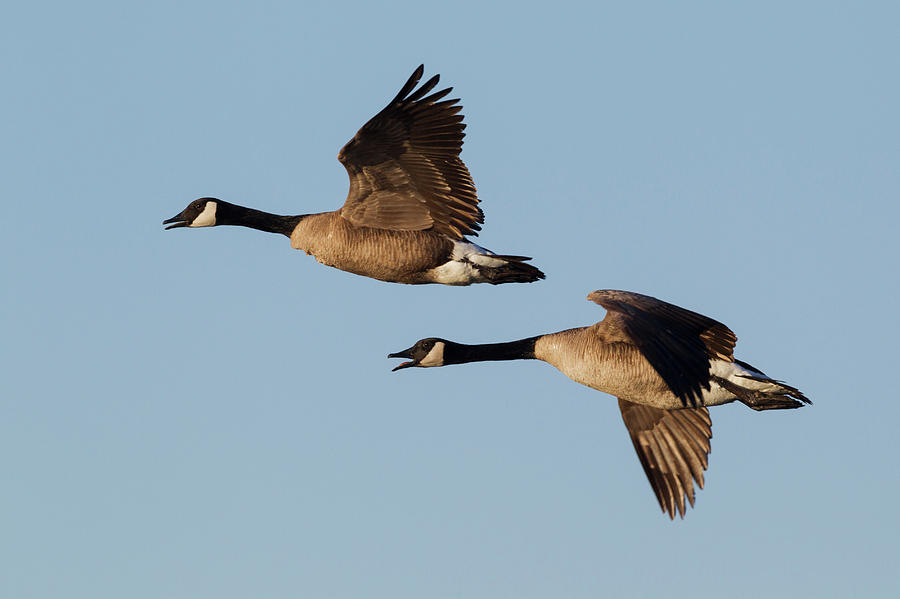
\includegraphics[width=0.5\textwidth,height=\textheight]{Images/Cover1.jpg}

\section*{Einleitung}\label{einleitung}
\addcontentsline{toc}{section}{Einleitung}

Korrelationen spielen eine zentrale Rolle in der Statistik und in vielen wissenschaftlichen Disziplinen. Sie ermöglichen es uns, Zusammenhänge zwischen zwei oder mehr Variablen zu quantifizieren und zu interpretieren.

Dieses Skriptum frischt Ihre bestehenden Grundkenntnisse über Korrelation auf und vertieft Ihr Verständnis der verschiedenen Korrelationstechniken. Ziel ist es, Ihnen die Werkzeuge an die Hand zu geben, um komplexe Datenbeziehungen zu analysieren und fundierte Schlussfolgerungen zu ziehen.

\section*{Variabilität}\label{variabilituxe4t}
\addcontentsline{toc}{section}{Variabilität}

Bevor wir uns mit einzelnen Techniken und Verfahren der linearen Modellbildung auseinandersetzen, soll in einem kurzen Exkurs eines der grundlegensten Prinzipien der statistischen Modellbildung wiederholt und diskutiert werden - die \emph{Varianz} von beobachten Werten.

Eigentlich ist es die Variabilität von Merkmalen, die statistische Methoden für die Erklärung von Effekten überhaupt erst auf den Plan ruft. Würden Merkmale wie z.B. Leistung einer Person, Persönlichkeitsmerkmale, Wetter, Produktionsgenauigkeit etc. nicht schwanken/variieren, würden wir heute nicht in diesem Raum sitzen und uns mit statistischen Modellen beschäftigen.

Der Begriff Variabilität ist für uns so alltäglich, dass wir ganz selbstverständlich damit umgehen. Doch was steckt wirklich dahinter? Wie können wir Sie nutzen um komplexere Eigenschaften einer Sache oder eines unerklärlichen Phenomäns auf die Spur zu kommen?

Betrachten wir zunächst einmal ein sehr einfaches Beispiel. In den nachfolgenden Graphen sind (sehr vereinfacht) mehrere Möglichkeiten dargestellt, wie eine Person mitsamt Hund sich entlang einer Straße bewegt.

\begin{figure}
\centering
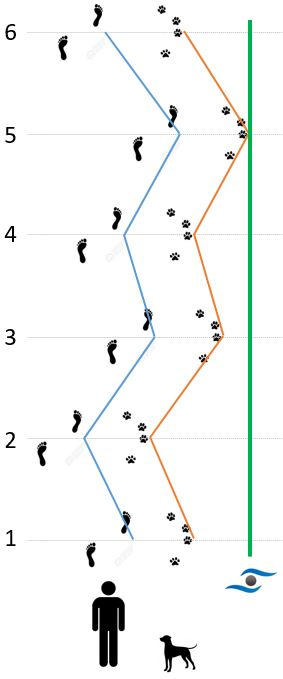
\includegraphics[width=0.25\textwidth,height=\textheight]{Images/GassiPositiveKorrelation.JPG}
\caption{\textbf{Abbildung 1}: Gassi gehen mit \emph{Blindenhund}. Die blaue Linie beschreibt den Weg des Hundehalters, die Orange den des Hundes. Die Grüne Line ist die Referenzlinie, von welcher aus der Abstand zur jeweiligen Position (Hund und Mensch) zu sechs Beobachtungszeitpunkten gemessen wurde.}
\end{figure}

Die Daten der Messungen sind in folgender Tabelle gegeben:

\begin{longtable}[]{@{}
  >{\centering\arraybackslash}p{(\columnwidth - 14\tabcolsep) * \real{0.1250}}
  >{\centering\arraybackslash}p{(\columnwidth - 14\tabcolsep) * \real{0.0972}}
  >{\centering\arraybackslash}p{(\columnwidth - 14\tabcolsep) * \real{0.1389}}
  >{\centering\arraybackslash}p{(\columnwidth - 14\tabcolsep) * \real{0.1111}}
  >{\centering\arraybackslash}p{(\columnwidth - 14\tabcolsep) * \real{0.0972}}
  >{\centering\arraybackslash}p{(\columnwidth - 14\tabcolsep) * \real{0.1389}}
  >{\centering\arraybackslash}p{(\columnwidth - 14\tabcolsep) * \real{0.1111}}
  >{\centering\arraybackslash}p{(\columnwidth - 14\tabcolsep) * \real{0.1111}}@{}}
\toprule\noalign{}
\begin{minipage}[b]{\linewidth}\centering
Mensch
\end{minipage} & \begin{minipage}[b]{\linewidth}\centering
Hund
\end{minipage} & \begin{minipage}[b]{\linewidth}\centering
MenschD
\end{minipage} & \begin{minipage}[b]{\linewidth}\centering
HundD
\end{minipage} & \begin{minipage}[b]{\linewidth}\centering
KP
\end{minipage} & \begin{minipage}[b]{\linewidth}\centering
ZMensch
\end{minipage} & \begin{minipage}[b]{\linewidth}\centering
ZHund
\end{minipage} & \begin{minipage}[b]{\linewidth}\centering
ZKP
\end{minipage} \\
\midrule\noalign{}
\endhead
\bottomrule\noalign{}
\endlastfoot
4 & 3 & 0.83 & 1 & 0.83 & 0.71 & 0.71 & 0.5 \\
5 & 4 & 1.83 & 2 & 3.66 & 1.56 & 1.42 & 2.22 \\
2 & 1 & -1.17 & -1 & 1.17 & -1 & -0.71 & 0.71 \\
3 & 2 & -0.17 & 0 & 0 & -0.15 & 0 & 0 \\
2 & 0 & -1.17 & -2 & 2.34 & -1 & -1.42 & 1.42 \\
3 & 2 & -0.17 & 0 & 0 & -0.15 & 0 & 0 \\
\end{longtable}

\begin{itemize}
\tightlist
\item
  In obiger Tabelle zeigen die Spalten \emph{Mensch} und \emph{Hund} jeweils den Abstand zur gedachten Beobachtungslinie pro Beobachtungszeitpunkt.
\item
  Die Spalten \emph{MenschD} und \emph{HundD} ist jeweils die Differenz jeder Beobachtung zum jeweiligen Mittelwert aller Beobachtungen, also \(MD_i = M_i - \bar{M}\) und \(HD_i = H_i - \bar{H}\) mit \(i \in \{1,6\}\).
\item
  Die Spalte \emph{KP} zeigt das Kreuzprodukt, also \(KP_i = MD_i \cdot HD_i\) mit \(i \in \{1,6\}\).
\item
  Die Spalten \emph{ZMensch} und \emph{ZHund} entsprechen den \(z\)-transformierten Werten, also \(z_i^M = (M_i - \bar{M}) / sd(M)\) und \(z_i^H = (H_i - \bar{H}) / sd(H)\)) mit \(i \in \{1,6\}\).
\item
  Die Spalte \emph{ZKP} entspricht dem Kreuzprodukt der z-Transformierten Werte, also \(ZKP_i = ZM_i \cdot ZH_i\) mit \(i \in \{1,6\}\).
\end{itemize}

Statistische Kennwerte für obige Daten (Mittelwert, Varianz und Standardabweichung) sind in folgender Tabelle dargestellt:

\begin{longtable}[]{@{}
  >{\centering\arraybackslash}p{(\columnwidth - 16\tabcolsep) * \real{0.1375}}
  >{\centering\arraybackslash}p{(\columnwidth - 16\tabcolsep) * \real{0.1125}}
  >{\centering\arraybackslash}p{(\columnwidth - 16\tabcolsep) * \real{0.1000}}
  >{\centering\arraybackslash}p{(\columnwidth - 16\tabcolsep) * \real{0.1250}}
  >{\centering\arraybackslash}p{(\columnwidth - 16\tabcolsep) * \real{0.1000}}
  >{\centering\arraybackslash}p{(\columnwidth - 16\tabcolsep) * \real{0.1000}}
  >{\centering\arraybackslash}p{(\columnwidth - 16\tabcolsep) * \real{0.1250}}
  >{\centering\arraybackslash}p{(\columnwidth - 16\tabcolsep) * \real{0.1000}}
  >{\centering\arraybackslash}p{(\columnwidth - 16\tabcolsep) * \real{0.1000}}@{}}
\toprule\noalign{}
\begin{minipage}[b]{\linewidth}\centering
~
\end{minipage} & \begin{minipage}[b]{\linewidth}\centering
Mensch
\end{minipage} & \begin{minipage}[b]{\linewidth}\centering
Hund
\end{minipage} & \begin{minipage}[b]{\linewidth}\centering
MenschD
\end{minipage} & \begin{minipage}[b]{\linewidth}\centering
HundD
\end{minipage} & \begin{minipage}[b]{\linewidth}\centering
KP
\end{minipage} & \begin{minipage}[b]{\linewidth}\centering
ZMensch
\end{minipage} & \begin{minipage}[b]{\linewidth}\centering
ZHund
\end{minipage} & \begin{minipage}[b]{\linewidth}\centering
ZKP
\end{minipage} \\
\midrule\noalign{}
\endhead
\bottomrule\noalign{}
\endlastfoot
\textbf{Mean} & 3.167 & 2 & -0.003 & 0 & 1.333 & -0.005 & 0 & 0.808 \\
\textbf{Var} & 1.367 & 2 & 1.367 & 2 & 2.052 & 0.997 & 1.008 & 0.756 \\
\textbf{SD} & 1.169 & 1.414 & 1.169 & 1.414 & 1.433 & 0.998 & 1.004 & 0.869 \\
\end{longtable}

Wenn also ein Hund jeder Bewegung der Person folgt und dabei auch stets denselben Abstand hält, sind deren beobachteten Pfade zwar örtlich gesehen unterschiedlich, aber die Varianz des einen erklärt vollständig die Varianz des anderen Pfades. Mit anderen Worten, die beiden Pfade zeigen eine perfekte Kovariation. Formal wird diese \emph{Kovariation} als \emph{durchschnittliche Summe der Kreuzprodukte} ermittelt, also (M = Mensch, H = Hund):

\(cov(M, H) = \frac{\sum_{i=1}^{6} (M_i - \bar{M}) \cdot (H_i - \bar{H})}{N-1} = 1.60\)

Setzt man die Beispieldaten in diese Berechnungsvorschrift ein, erhält man für die Summe der Kreuzprodukte 8. Die Kovarianz der beobachteten Werte ist (als durchschnittliche Kreuzproduktsumme) somit \(cov(M,H) =\) 1.6. Die Korrelation berechnet sich dann ganz einfach zu:

\(r(M, H) = \frac{cov(M,H)}{s_M \cdot s_H} = \frac{1.6}{1.169 \cdot 1.414} = 0.968 \simeq 1\)

Im vorliegenden Beispiel ergibt sich eine Korrelation \(r(M,H) =\) 0.97 (also eine positive und perfekte Korrelation).

Der Korrelationskoeffizient hat gegebüber der Kovarianz den Vorteil, dass er durch die Normierung über die Standardabweichungen:

\begin{enumerate}
\def\labelenumi{\arabic{enumi}.}
\tightlist
\item
  einen (einheitenlosen) Wertebereich zwischen \(r \in [-1, 1]\) aufweist und damit vergleichbar mit anderen Korrelationswerten wird.
\item
  Als praktische \textbf{Effektgröße} interpretiert werden kann.
\item
  Das Quadrat des Korrelationskoeffizienten (\(r^2\), auch \textbf{Varianzaufklärung}, \textbf{Determinationskoeffizient} genannt) Auskunft über die aufgeklärte Varianz gibt.
\end{enumerate}

Letzteres Maß spielt eine wesentliche Rolle sowohl bei der Korrelationsanalyse, als auch bei der multiplen Regression und anderen Verfahren.

Die Bedeutung der Kovarianu sei anhand des verwendeten Beispiels nochmals verdeutlicht:

\begin{quote}
Im Fall einer perfekten Kovarianz (also 100\% Übereinstimmung der Bewegungen von Mensch und Hund), braucht man nur mehr die Bewegung einer Variablen zu wissen (z.B. die des Menschen), um die Bewegungen des Hundes zu bestimmen (erklären). Somit erklärt die Variabilität der Bewegung vom Menschen zu 100 \% die Variabilität der Bewegungen des Hundes.
\end{quote}

Die Beziehung zwischen zwei (intervallskallierten) Variablen lässt sich am besten mit einem Streudiagramm darstellen:

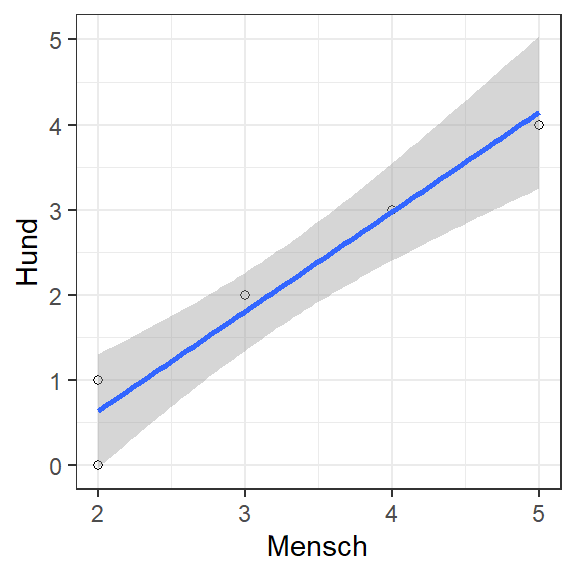
\includegraphics{01_Korrelationen_files/figure-latex/Gassi_Pos_Korr_Scatter-1.pdf}

Die folgende Abbildung zeigt ein weiteres Mensch-Hund Beispiel:

\begin{figure}
\centering
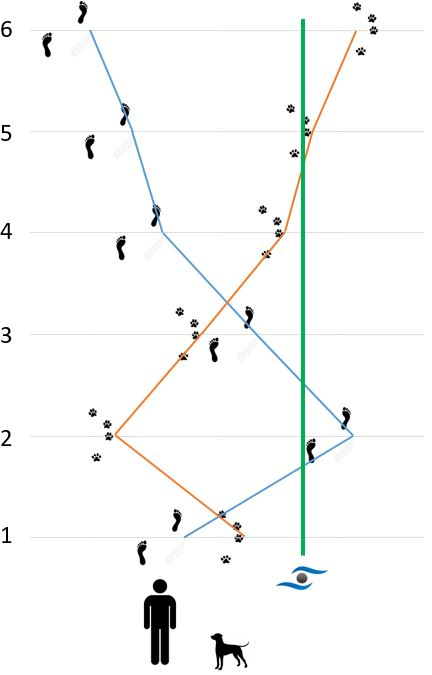
\includegraphics[width=0.25\textwidth,height=\textheight]{Images/GassiNegativeKorrelation.JPG}
\caption{\textbf{Abbildung 2}: in diesem Beispiel scheint es sich um eine Hund zu handeln, der bestmöglich das Gegenteil vom Menschen macht. Bestmöglich dahingehen, dass er nicht nur in die genau entgegengesetzte Richtung ausweicht, sondern dabei auch auf den genauen Abstand der Abweichung achtet.}
\end{figure}

In diesem Fall ist die Korrelation auch perfekt, nur eben in die entgegengesetzte Richtung, was zur Folge hat, dass diese Korrelation den Wert \(r(M,H) = -1\) zeigt.

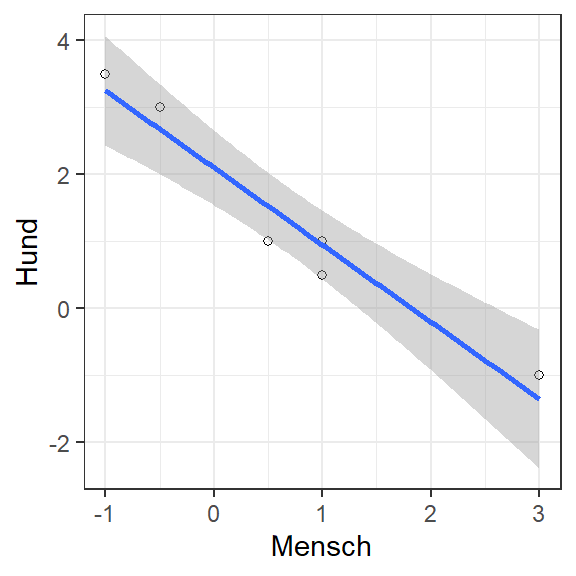
\includegraphics{01_Korrelationen_files/figure-latex/Gassi_Neg_Korr_Scatter-1.pdf}

Interessant und der Praxis am ehesten entsprechend, sind jedoch Fälle, in denen zwei Variablen nur teilweise Gemeinsamkeiten aufweisen. Im folgenden Beispiel wäre

\begin{figure}
\centering
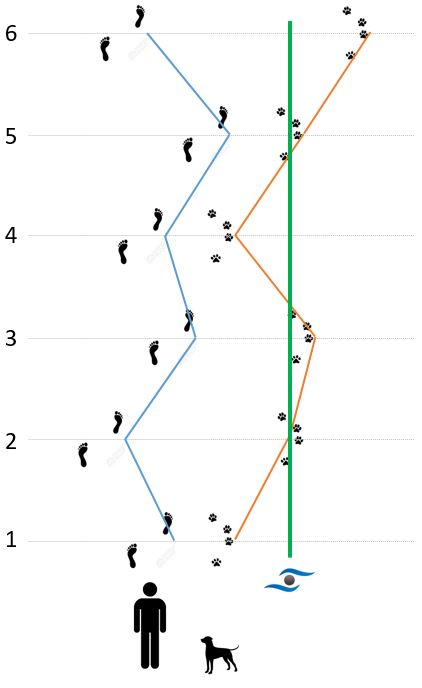
\includegraphics[width=0.25\textwidth,height=\textheight]{Images/GassiBeliebigeKorrelation.JPG}
\caption{\textbf{Abbildung 3}: Hund und Mensch bewegen sich zum Teil unabhängig, zum Teil aber auch synchron. Dies entspricht dann einer Kovarianz, bzw. Korrelation die irgendwo zwischen \(r \in [-1, 1]\) liegt (im Beispiel ist \(r(M,H) = 0.5\) und somit \(r^2 = 0.25\)).}
\end{figure}

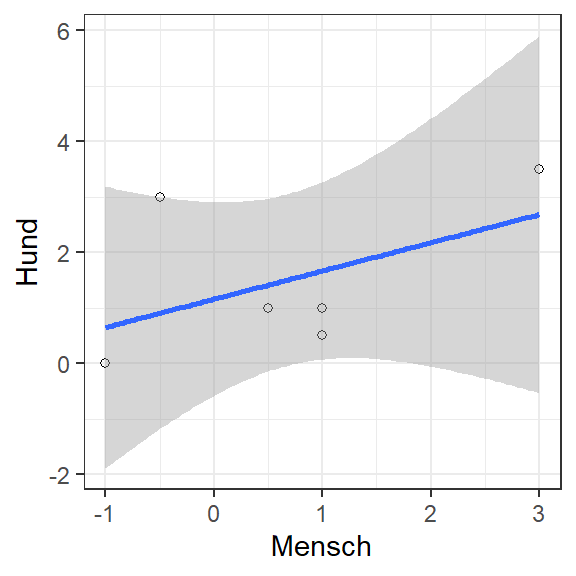
\includegraphics{01_Korrelationen_files/figure-latex/Gassi_Teilweis_Korr_Scatter-1.pdf}

Die Korrelation liegt in diesem Beispiel bei \(r(M,H) = 0.5\). Daraus lässt sich auch nochmals eine sehr wichtige Erkenntnis bezüglich der geteilten Varianz der beiden Variablen festhalten:

\begin{quote}
Bei einer Korrelation von \(r(x,y) = 0.5\) entspricht der Determinationskoeffizient \(r^2(x,y) = 0.25\). In Prozent ausgedrückt, werden als 25\% der Variabilität einer Variablen (z.B. Hund) durch die Variable Mensch erklärt. In welchen Abschnitten der Daten diese gemeinsame Variablität auftritt, lässt sich durch den \(r\) nicht bestimmen.
\end{quote}

Diese Feststellung führt uns aber zu einer weiteren Betrachtung von Variablitäten:

\begin{figure}
\centering
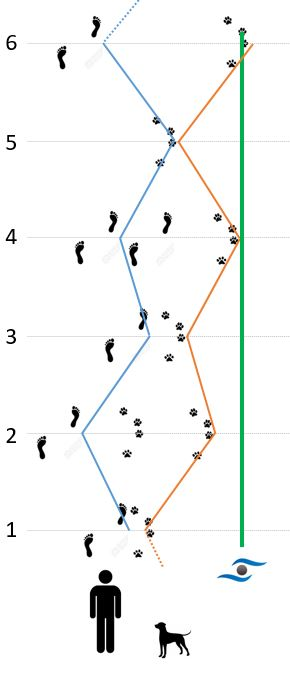
\includegraphics[width=0.25\textwidth,height=\textheight]{Images/GassiAutokorrKorrelation.JPG}
\caption{\textbf{Abbildung 4}: Hund und Mensch scheinen sich wieder synchron, aber in gegenseitiger Richtung zu bewegen. Man würde also eine negative und hohe Korrelation erwarten. Interressant ist jedoch die Beobachtung, dass ein Versatz der Beobachtungen um eine Einheit zu einem hohen positiven Zusammenhang führen würde!}
\end{figure}

Würde man davon ausgehen, dass sich der Mensch und Hund bei jedem Messzeitpunkt (1 bis 6) jeweils auf der gleichen Höhe befunden haben, dann wird man eine hohe \textbf{negative Korrelation} erhalten. Nimmt man jedoch an, dass der Mensch zum Messzeitpunkt (MZP) 1, der Hund aber bereits auf MZP 2 war, dann verschiebt sich die Spur des Hundes einfach um einen MZP nach oben! Korreliert man nun diese beiden Beobachtungen, würde sich eine nahezu perfekte \textbf{positive Korrelation} ergeben!

\begin{quote}
Durch schrittweises Verschieben der Werte einer Variablen um eine Einheit (\(\tau_i\)) mit anschließender Berechnung der Korrelationskoeffizienten (\(r_{\tau_i}(x,y)\)), erhält man in Abhängigkeit von der Anzahl der Verschiebungen (\(i \in [0, N-1]\)) maximal \(N\) neue Korrelatinskoeffizienten. Man bezeichnet diese Art der Korrelationsberechnung als \textbf{Kreuzkorrelation}.
\end{quote}

Für das Beispiel ergibt sich eine normale Korrelation von \(r(M,H)=\) -1. Die Korrelationen berechnet nach dem Versatzprinzip ergeben folgendes Bild:

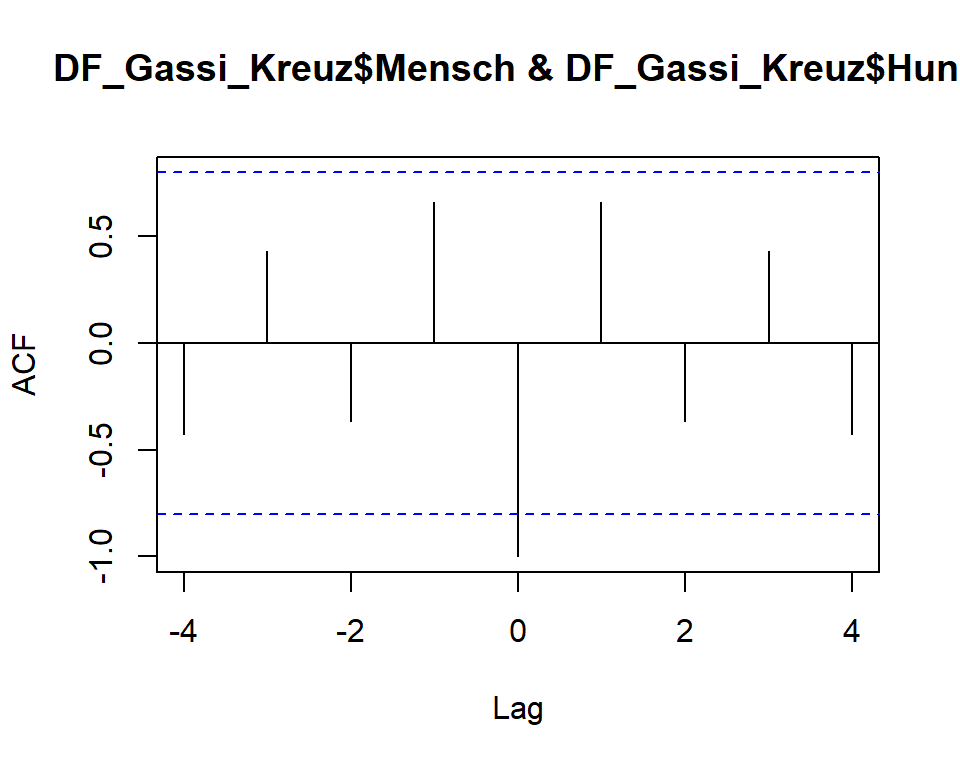
\includegraphics{01_Korrelationen_files/figure-latex/Gassi_Kreuz_Korr_Plot-1.pdf}

Die Verschiebung \(\tau\) wurde in diesem Beispiel mit \(i = 4\) angegeben, d.h. es wurden die Werte der Variablen Hund um jeweils vier Schritte nach links und vier Schritte nach rechts verschoben. Bei jeder Verschiebung wurde die Korrelation berechnet (im Graphen ist die Verschiebung mit \emph{Lag} auf der x-Achse angegeben). Auf der y-Achse wird der entsprechende Korrelationskoeffient angezeigt.

\begin{longtable}[]{@{}
  >{\centering\arraybackslash}p{(\columnwidth - 2\tabcolsep) * \real{0.0833}}
  >{\centering\arraybackslash}p{(\columnwidth - 2\tabcolsep) * \real{0.1667}}@{}}
\toprule\noalign{}
\begin{minipage}[b]{\linewidth}\centering
Tau
\end{minipage} & \begin{minipage}[b]{\linewidth}\centering
CrossCorr
\end{minipage} \\
\midrule\noalign{}
\endhead
\bottomrule\noalign{}
\endlastfoot
-4 & -0.4253 \\
-3 & 0.431 \\
-2 & -0.3678 \\
-1 & 0.6609 \\
0 & -1 \\
1 & 0.6609 \\
2 & -0.3678 \\
3 & 0.431 \\
4 & -0.4253 \\
\end{longtable}

Die Werte der Tabelle zeigen nochmals den krassen Wechsel der Korrelation zwischen den Werte \(\tau = 0\) (also keiner Verschiebung) und \(\tau = 1\). Werden die Werte um nur einen Beobachtungspunkt verschoben, ändert sich die Korrelation von einer perfekt negativen, zu einer sehr hohen positiven Korrelation!

Eine weitere wichtige Eigenschaft die mit Hilfe dieser Vorgehensweise geprüft werden kann, ist die der sogenannten \textbf{Autokorrelation}. Diese funktioniert im Prinzip wie die eben beschriebene Kreuzkorrelation, mit dem Unterschied, dass eine Variable mit verschobenen ``Eigenversionen'' korreliert wird. Folgendes Beispiel zeigt das Ergebnis für die Variable Mensch unseres Beispiels:

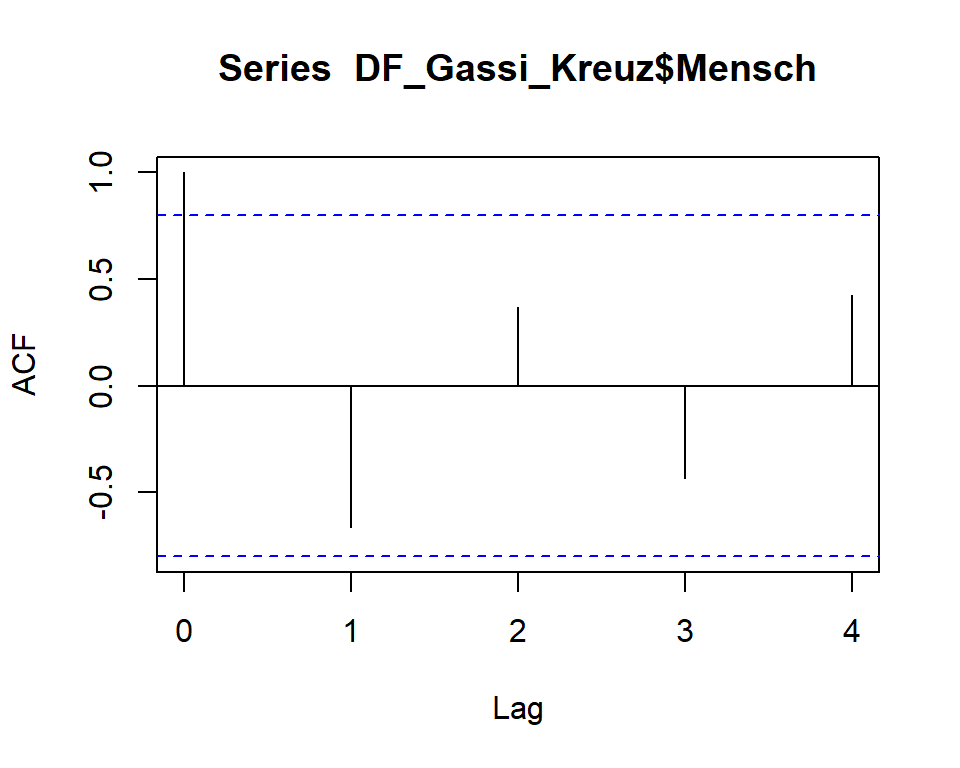
\includegraphics{01_Korrelationen_files/figure-latex/Gassi_Auto_Korr_Plot-1.pdf}

Die Verschiebung \(\tau\) wurde in diesem Beispiel mit \(i = 4\) angegeben, d.h. es wurden die Werte der Variablen Mensch ebenfalls schrittweise in eine Richtung verschoben. Bei jeder Verschiebung wurde die Korrelation berechnet (im Graphen ist die Verschiebung mit \emph{Lag} auf der \(x\)-Achse angegeben). Auf der \(y\)-Achse wird der entsprechende Korrelationskoeffient angezeigt.

\begin{longtable}[]{@{}
  >{\centering\arraybackslash}p{(\columnwidth - 2\tabcolsep) * \real{0.0833}}
  >{\centering\arraybackslash}p{(\columnwidth - 2\tabcolsep) * \real{0.1667}}@{}}
\toprule\noalign{}
\begin{minipage}[b]{\linewidth}\centering
Tau
\end{minipage} & \begin{minipage}[b]{\linewidth}\centering
CrossCorr
\end{minipage} \\
\midrule\noalign{}
\endhead
\bottomrule\noalign{}
\endlastfoot
0 & 1 \\
1 & -0.6609 \\
2 & 0.3678 \\
3 & -0.431 \\
4 & 0.4253 \\
\end{longtable}

Die perfekte positive Korrelation bei einer Verschiebung um den Wert \(\tau = 0\) ist bei der Autokorrelation trivial, da es sich ja um einen direkten Vergleich der Variablen mit sich selbst handelt. Bei Lag = 1 wird jedoch ersichtlich, dass sich die Korrelation ändert (auf \(r = -0.66\)), springt dann wieder auf \(r = +0.37\) usw.

Es ist zu beachten, dass dieser Datensatz nur zu Demonstrationszwecken erzeugt wurde. Eine inhaltliche Interpretation wäre im gegebenen Fall nicht angebracht.

Nichts desto trotz sollte durch diese Beispiel gezeigt werden, dass sowohl die Kreuzkorrelation als auch die Autokorrelation vor allem in der Zeitreihenanalyse (und damit auch bei Längsschnittstudien) wichtige Erkenntnisse über die betrachteten Variablen liefern können. Vor allem kann eine vorliegende \textbf{Autokorrelation} bei der MLR zu beträchtlichen Einschränkungen der Gültigkeit einen Modells beitragen. Bei den MLR-Methoden werden wir noch über Möglichkeiten sprechen, Autokorrelationen auf statitische Signifikanz zu prüfen (Stichwort: \href{https://en.wikipedia.org/wiki/Durbin\%E2\%80\%93Watson_statistic}{Durbin-Watson}).

\section*{Korrelationen}\label{korrelationen}
\addcontentsline{toc}{section}{Korrelationen}

Korrelationen sind ein Maß für den statistischen Zusammenhang zweier Datenreihen. Ein Korrelationsmaß impliziert daher auch stochastische Abhängigkeit - ohne jedoch auf kausale Zusammenhänge schließen zu können.

Korrelationen werden i.A. der \emph{deskriptiven Statistik} zugeordnet. Durch eine Reihe von Verfahren, wie z.B. partielle Korrelation, multiple Korrelation oder Faktorenanalyse, kann die einfache Korrelation zweier Variablen auf Beziehungen zwischen zwei Variablen unter Berücksichtigung des Einflusses weiterer Variablen werden.

Korrelationen sind ein unverzichtbares Werkzeug für viele Forschungsgebiete und stehen häufig am Beginn jeder weiteren Datenanalyse, wie z.B.:

\begin{itemize}
\tightlist
\item
  multiple Regression
\item
  Faktorenanalyse
\item
  Clusteranalyse
\item
  Mediator- und Moderator-Analyse
\end{itemize}

\subsection*{Pearson Produkt Moment Korrelation}\label{pearson-produkt-moment-korrelation}
\addcontentsline{toc}{subsection}{Pearson Produkt Moment Korrelation}

Die häufigst verwendete Form der Korrelationsberechnung ist die Pearson-Produkt-Moment Korrelation. Bei dieser Methode wird die Beziehung zwischen zwei metrische Variablen (bzw. eine metrische und eine dichotome Variable) als Kennzahl mit dem Wertebereich \(r \in [-1,1]\) berechnet.

Die Berechnung einer Korrelation ist für sich gesehen an keine Voraussetzungen gebunden. Hingegen fordern eine sinnvolle Interpretationen der berechneten Kennwerte und vor allem die statistischen Tests von Korrelationskoeffizienten folgende inhaltliche und formale Überlegungen:

\begin{itemize}
\tightlist
\item
  \textbf{Skalenniveau}: der Korrelationskoeffizient liefert sinnvoll interpretierbare Ergebnisse wenn die Variablen mindestens intervallskaliert sind (oder für eine intervallskalierte und eine dichotome Variable\footnote{dieser Spezialfall ist unter biserialer, bzw. punktbiserialer Korrelation bekannt.}).
\end{itemize}

\begin{itemize}
\tightlist
\item
  \textbf{Endliche Varianz (und Kovarianz)}: bei Erhöhung des Stichprobenumfangs darf sich die Variabilität nicht immer weiter erhöhen, sondern sollte sich stabilisieren. Bei Variablen, die bivariat normalverteilt sind, ist diese Voraussetzung automatisch gegeben. Der Korrelationskoeffizient ist damit auch gleichzeitig der \emph{Maximum-Likelyhood Schäzter} des Korrelationskoeffizienten in der Grundgesamtheit (asymptotisch \emph{erwartungstreu} und \emph{effizient}).
\end{itemize}

\begin{figure}
\centering
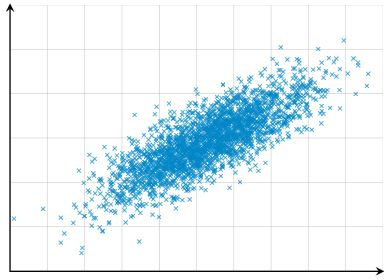
\includegraphics[width=0.4\textwidth,height=\textheight]{Images/EndlicheVarianz.JPG}
\caption[\textbf{Abbildung 5}: Endliche Varianz]{\textbf{Abbildung 5}: Endliche Varianz\footnotemark{}}
\end{figure}
\footnotetext{\href{https://matheguru.com/stochastik/korrelation-korrelationskoeffizient.html}{die Abbildungen wurden der Website Matheguru entnommen}}

\begin{itemize}
\tightlist
\item
  \textbf{Linearität}: die Korrelation ist ein Maß für \textbf{lineare Abhängigkeit}. Abweichungen der Daten von dieser Linearitätsannahme führen zu einer mehr oder weniger starken Verzerrung des Korrelationskoeffizienten, wie in den nachfolgenden Beispielen gezeigt wird:
\end{itemize}

\begin{figure}
\centering
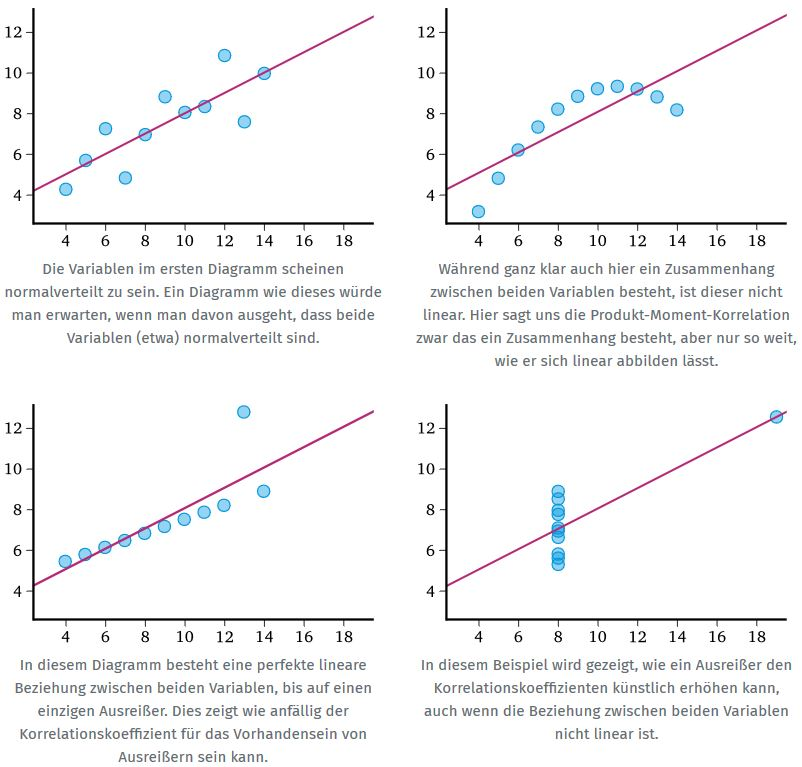
\includegraphics[width=0.6\textwidth,height=\textheight]{Images/Linearitaet.JPG}
\caption{\textbf{Abbildung 6}: Linearität und Korrelation}
\end{figure}

Vor allem zur Prüfung der Signifikanz einer Korrelation sollem man weitere Voraussetzungen überprüfen:

\begin{itemize}
\item
  \textbf{Normalverteilung}: Korrelation berechnen sich aus dem Kreuzprodukt von z-standardisierten Werten zweier Variablen. Für diese Berechnung wird der Mittelwert als zentraler Kennwert verwendet, welcher nur dann ein ``sinnvoller'' Kennwert für die Daten ist, wenn diese zumindest symmetrisch und im besten Fall normalverteilt sind.
\item
  \textbf{Homoskedastizität}: bedeutet gleichmäßige Streuung der Daten zweier (exogene und endogene) Variablen. Sind die exogene und die endogene Variable\footnote{eine \emph{exogene} Variable ist eine erklärende Variable, die mit der Störgröße unkorreliert ist (sogenannte Exogenität). Eine \emph{endogene} Variable in einem multiplen Regressionsmodell ist eine erklärende Variable, die entweder aufgrund einer ausgelassenen Variablen, eines Messfehlers oder wegen Simulatanität mit der Störgröße korreliert ist (sogenannte Endogenität).} nicht mehr identisch verteilt, d.h. sie ändern ihre Variablität mit zu/abnehmenden Werten einer Variablen, spricht man von \textbf{Herteroskedastizität}. Das hat zur Folge hat, dass die KQ\footnote{KQ steht für kleinste Quadrate (auch MLS - Minimum Least Square, oder OLS - Ordinary Least Square) und ist eine einfache Schätzung über minimierte quadradische Abstände der Residuen (Fehler) zu einem Modell (Mittelwert, Gerade, etc.)}-Schätzer nicht mehr effizient sind und der Standardfehler der Koeffizienten verzerrt und nicht konsistent wird.
\end{itemize}

\begin{figure}
\centering
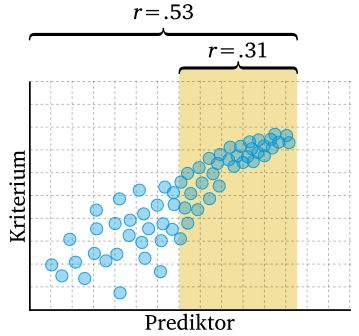
\includegraphics[width=0.3\textwidth,height=\textheight]{Images/Variabilitaet.JPG}
\caption{\textbf{Abbildung 7}: Variablität(einschränkung) und Korrelation}
\end{figure}

\begin{itemize}
\tightlist
\item
  \textbf{KEINE Ausreißer}: der Korrelationskoeffizient ist nicht robust gegenüber Ausreißern. Dies bedeutet, dass Ausreißer den Korrelationskoeffizienten sowohl künstlich erhöhen als auch künstlich senken können.
\end{itemize}

\begin{figure}
\centering
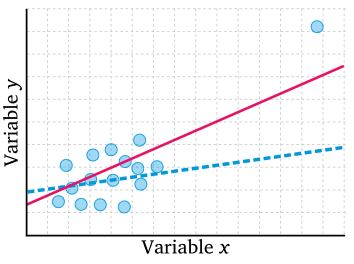
\includegraphics[width=0.3\textwidth,height=\textheight]{Images/Ausreisser.JPG}
\caption{\textbf{Abbildung 8}: Einfluss von Ausreißer bei linearer Modellbildung}
\end{figure}

\begin{itemize}
\tightlist
\item
  \textbf{KEINE Kluster}: es kann vorkommen, dass zwei oder mehr Gruppen eine Korrelation zeigen, die eigentlich getrennt untersucht werden müssten. Dieses Problem wird oft auch mittels \textbf{partieller Korrelation} umgangen, bei der mögliche Drittvariablen statistisch konstant gehalten werden.
\end{itemize}

\begin{figure}
\centering
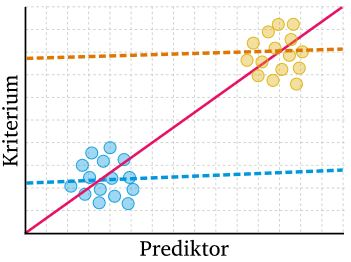
\includegraphics[width=0.3\textwidth,height=\textheight]{Images/Cluster.JPG}
\caption{\textbf{Abbildung 9}: Kluster und deren Auswirkung bei linearer Modellierung}
\end{figure}

\subsubsection*{Beispiel Pearson Korrelation}\label{beispiel-pearson-korrelation}
\addcontentsline{toc}{subsubsection}{Beispiel Pearson Korrelation}

Im folgenden, fiktiven Beispiel werden die Zusammenhänge von Klausurperformanz (\emph{EP}), Intelligenz (\emph{IQ}), Vorbereitungszeit (\emph{VZ}) und Prüfungsangst (\emph{PA}) korreliert. Der Code zum Laden der Daten sowie die Daten selbst sind in nachfolgender Ausgabe/Tabelle dargestellt:

\begin{Shaded}
\begin{Highlighting}[]
    \FunctionTok{load}\NormalTok{(}\StringTok{"Daten/CorrBsp1.Rda"}\NormalTok{)}
\end{Highlighting}
\end{Shaded}

\begin{longtable}[]{@{}
  >{\centering\arraybackslash}p{(\columnwidth - 6\tabcolsep) * \real{0.0694}}
  >{\centering\arraybackslash}p{(\columnwidth - 6\tabcolsep) * \real{0.0833}}
  >{\centering\arraybackslash}p{(\columnwidth - 6\tabcolsep) * \real{0.0694}}
  >{\centering\arraybackslash}p{(\columnwidth - 6\tabcolsep) * \real{0.0833}}@{}}
\toprule\noalign{}
\begin{minipage}[b]{\linewidth}\centering
EP
\end{minipage} & \begin{minipage}[b]{\linewidth}\centering
IQ
\end{minipage} & \begin{minipage}[b]{\linewidth}\centering
VZ
\end{minipage} & \begin{minipage}[b]{\linewidth}\centering
PA
\end{minipage} \\
\midrule\noalign{}
\endhead
\bottomrule\noalign{}
\endlastfoot
74 & 109 & 16 & 117 \\
67 & 96 & 18 & 122 \\
72 & 106 & 13 & 108 \\
66 & 89 & 12 & 97 \\
63 & 93 & 14 & 98 \\
67 & 102 & 15 & 106 \\
\end{longtable}

\subsubsection*{Aufgabe Korrelation}\label{aufgabe-korrelation}
\addcontentsline{toc}{subsubsection}{Aufgabe Korrelation}

Kopiere den obigen Code zum Laden der Daten in eine R-Script-Datei. Führe nun folgende Aufgaben aus:

\begin{enumerate}
\def\labelenumi{\arabic{enumi}.}
\tightlist
\item
  Ermittle mit einer geeigneten Funktion die Korrelationen und prüfe diese auch auf statistische Signifikanz.
\item
  Zeichne einen Korrelationsplot mit dem Paket \emph{corrplot}.
\item
  Berechne die Teststärke der Korrelation \(r(IQ, EP)\) (\emph{Hinweis}: verwende die Funktion \emph{pwr.r.test} des Pakets \emph{pwr}).
\item
  Verwende diese Funktion (\emph{pwr.r.test}) um für eine Korrelation \(r(x,y) = 0.21\) den optimalen Stichprobenumfang zu berechnen.
\item
  Prüfe mit Hilfe der Funktion \emph{mvn} aus dem Paket \emph{MVN} die Voraussetzung der bivariaten Normalverteilung der Variablenpaare (EP,IQ), (EP, VZ) und (EP,PA).
\item
  Berechne die durchschnittliche Korrelation von \(r_1(EP,IQ)\), \(r_1(EP,VZ)\) und \(r_1(EP,PA)\). Beachte, dass zur Berechnung von durchschnittlichen Korrelationswerten eine Fisher-Z-Transformation notwendig ist (\emph{Hinweis}: verwende die \emph{fisherz()} und \emph{fisherz2r()} des Pakets \emph{psych}).
\item
  Prüfe, ob der Unterschied der Korrelationskoeffizienten \(r(EP,IQ) = 0.47\) und \(r(EP,VZ) = 0.36\)
  statistisch signifikant ist. Verwende die Funktion \emph{paired.r()} aus dem Paket \emph{psych}.
\end{enumerate}

\hyperref[aufgabe-korrelation-lsg]{Lösung Aufgabe}

\subsection*{Kausalität}\label{kausalituxe4t}
\addcontentsline{toc}{subsection}{Kausalität}

Eine relevante (statistisch signifikante) Korrelation liefert keinen Beleg für die Kausalität. Vor allem in der Medizin und Psychologie suchen Forscher nach Kriterien für Kausalität. Es existieren mehrere Ansätze zur Erklärung der Ursächlichkeit einer Korrelation (siehe z.B. die 9 \href{https://de.wikipedia.org/wiki/\%C3\%84tiologie_(Medizin)}{Bradford-Hill-Kriterien}).

\subsection*{Partial- Semipartialkorrelation}\label{partial--semipartialkorrelation}
\addcontentsline{toc}{subsection}{Partial- Semipartialkorrelation}

Die \emph{partielle Korrelation} ist die bivariate Korrelation zweier Variablen, welche mittels linearer Regression vom Einfluss einer Drittvariablen bereinigt wurden.

Eine \emph{Semipartialkorrelation} ist ein Zusammenhang zwischen einer residualisierten und einer nicht-residualisierten Variable.

\begin{figure}
\centering
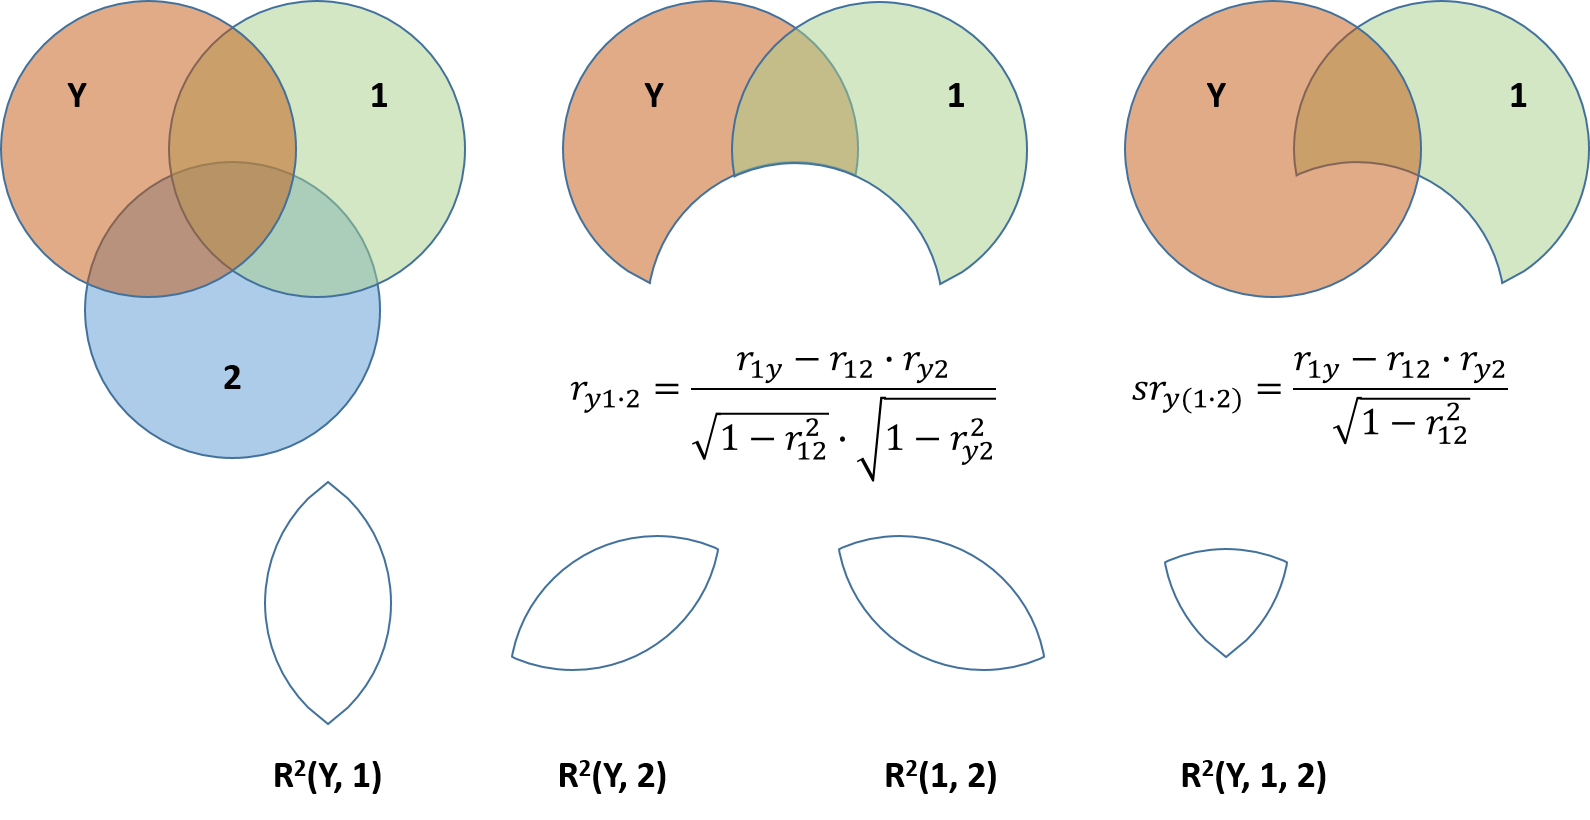
\includegraphics[width=0.8\textwidth,height=\textheight]{Images/PartialSemipartialkorrelation.png}
\caption{\textbf{Abbildung 10}: Partial und Semipartialkorrelation in einem Venn-Diagramm dargestellt}
\end{figure}

\subsubsection*{Beispiel Partial- Semipartialkorrelation}\label{beispiel-partial--semipartialkorrelation}
\addcontentsline{toc}{subsubsection}{Beispiel Partial- Semipartialkorrelation}

Folgendes Beispiel verdeutlicht die Wirkungsweise einer Partial- und Semipartialkorrelation. Kopier den folgenden Code in ein R-Script und führe diesen dann aus. Diskutiere die Ergebnisse.

\begin{Shaded}
\begin{Highlighting}[]
\NormalTok{    examData  }\OtherTok{\textless{}{-}} \FunctionTok{read.delim}\NormalTok{(}\StringTok{"Daten/Exam Anxiety.dat"}\NormalTok{, }\AttributeTok{header =} \ConstantTok{TRUE}\NormalTok{)}
\NormalTok{    examData2 }\OtherTok{\textless{}{-}}\NormalTok{ examData[, }\FunctionTok{c}\NormalTok{(}\StringTok{"Exam"}\NormalTok{, }\StringTok{"Anxiety"}\NormalTok{, }\StringTok{"Revise"}\NormalTok{)]}
    
    \CommentTok{\# Normale Korrelation}
\NormalTok{      pander}\SpecialCharTok{::}\FunctionTok{pander}\NormalTok{(}\FunctionTok{round}\NormalTok{(}\FunctionTok{cor}\NormalTok{(examData2),}\DecValTok{2}\NormalTok{))}
    \CommentTok{\# Partielle Korrelation}
      \CommentTok{\# library(ppcor)}
\NormalTok{      pander}\SpecialCharTok{::}\FunctionTok{pander}\NormalTok{(}\FunctionTok{round}\NormalTok{(ppcor}\SpecialCharTok{::}\FunctionTok{pcor}\NormalTok{(examData2)}\SpecialCharTok{$}\NormalTok{estimate,}\DecValTok{2}\NormalTok{))}
    \CommentTok{\# Partialkorrelation mit Linearen Modell    }
\NormalTok{      Mod1            }\OtherTok{\textless{}{-}} \FunctionTok{lm}\NormalTok{(Exam }\SpecialCharTok{\textasciitilde{}}\NormalTok{ Revise, }\AttributeTok{data =}\NormalTok{ examData2)}
\NormalTok{      Res\_Exam\_Rev    }\OtherTok{\textless{}{-}} \FunctionTok{residuals}\NormalTok{(Mod1)    }
\NormalTok{      Mod2            }\OtherTok{\textless{}{-}} \FunctionTok{lm}\NormalTok{(Anxiety }\SpecialCharTok{\textasciitilde{}}\NormalTok{ Revise, }\AttributeTok{data =}\NormalTok{ examData2)}
\NormalTok{      Res\_Anx\_Rev     }\OtherTok{\textless{}{-}} \FunctionTok{residuals}\NormalTok{(Mod2)    }
\NormalTok{      pr\_Exam\_Anx\_Rev }\OtherTok{\textless{}{-}} \FunctionTok{round}\NormalTok{(}\FunctionTok{cor}\NormalTok{(Res\_Exam\_Rev, Res\_Anx\_Rev), }\DecValTok{2}\NormalTok{)}
\end{Highlighting}
\end{Shaded}

In diesem Code wurde zur Veranschaulichung der Wirkungsweise einer Partial/Semipartialkorrelation eine lineare Regression verwendet. Was dabei genau passiert sei durch nachfolgende Abbildung nochmals veranschaulicht:

\begin{figure}
\centering
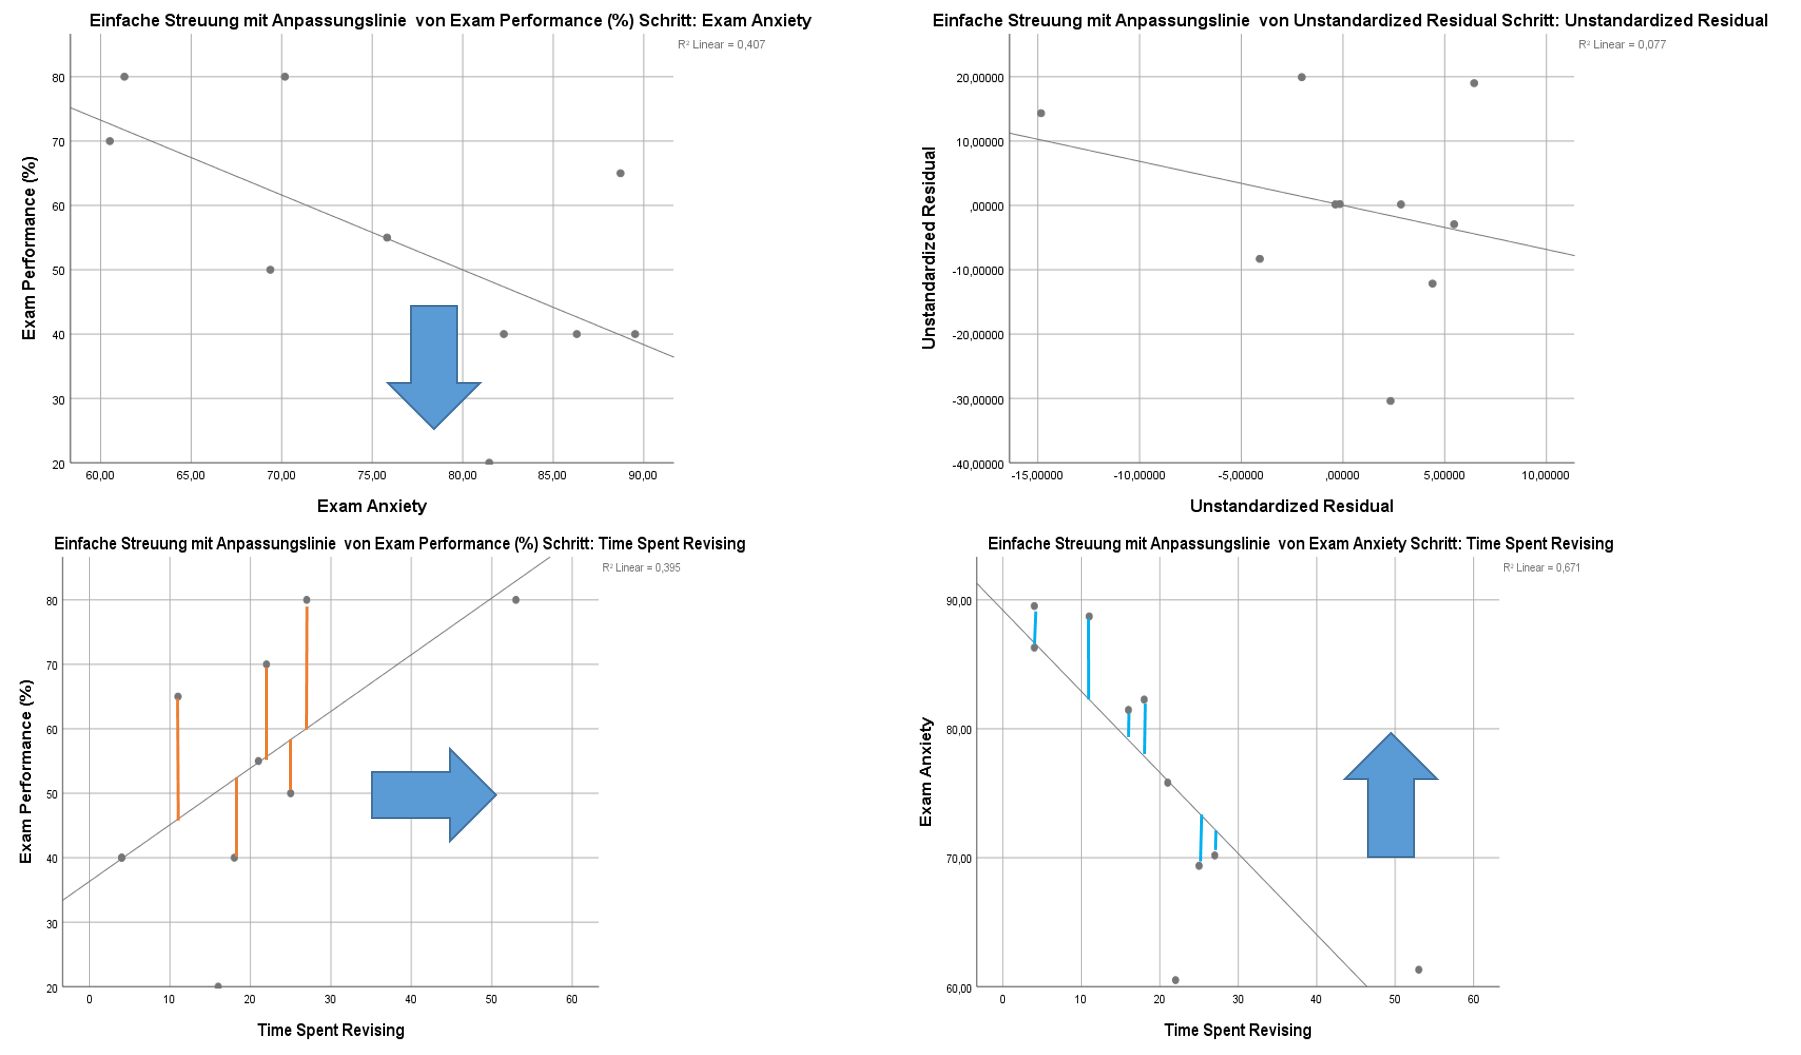
\includegraphics[width=1\textwidth,height=\textheight]{Images/PartialSemipartialLineareRegr.png}
\caption{\textbf{Abbildung 11}: Partialkorrelation als lineares Regressionsmodell. Für die Beziehung Examperformance und Exam Anxiety soll der Effekt von Revisiotime berücksichtigt werden. Die roten Linien entsprechen den Residuen der Regression Revisiontime mit Exam Performance. Die blauen den Residuen der Regression Revisiontime mit Exam Anxiety. Der linke obere Graph stellt die Beziehung von Anxiety und Examperfomance bereinigt von Revisiontime dar. Details siehe nachfolgendemn Text.}
\end{figure}

\begin{enumerate}
\def\labelenumi{\arabic{enumi}.}
\tightlist
\item
  Examperformance wird durch Revisiontime vorhergesagt. Die Residuen sind jener Anteil an Variabilität der Examperformanz, der nicht durch Revsiontime vorhergesagt werden können\footnote{anderenfalls würden ja alle beobachteten Werte auf der Gerade liegen!}. Diese über die durch Revisiontime erklärbare Variabilität von Examperformance kann zurückgeführt werden auf:

  \begin{itemize}
  \tightlist
  \item
    andere erklärende Merkmale, bzw.
  \item
    Messfehler
  \end{itemize}
\item
  Anxiety wird durch Revisiontime vorhergesagt. Auch hier gilt wieder, dass die Residuen der Variabilität von Anxiete, bereinigt von Revisiontime entsprechen.
\item
  Die Korrelation der Residuen entspricht nun genau der Partialkorrelation \(r_{Y1\cdot2}\)
\end{enumerate}

Bei der Semipartialkorrelation bereinigt man nun nicht beide Variablen, sonder eben nur einen Teil (z.B. wird nur die Anxiety von Revisiontime bereiningt).

Kopiere den nachfolgenden Code in ein R-Script und führe diesen aus. Diskutiere die Ergebnisse!

\begin{Shaded}
\begin{Highlighting}[]
    \CommentTok{\# Semipartielle Korrelation}
\NormalTok{      pander}\SpecialCharTok{::}\FunctionTok{pander}\NormalTok{(}\FunctionTok{round}\NormalTok{(ppcor}\SpecialCharTok{::}\FunctionTok{spcor}\NormalTok{(examData2)}\SpecialCharTok{$}\NormalTok{estimate,}\DecValTok{2}\NormalTok{))}
    \CommentTok{\# Semipartialkorrelation mit Linearen Modell    }
\NormalTok{      sr\_Exam\_Anx\_Rev }\OtherTok{\textless{}{-}} \FunctionTok{round}\NormalTok{(}\FunctionTok{cor}\NormalTok{(examData2}\SpecialCharTok{$}\NormalTok{Exam, Res\_Anx\_Rev), }\DecValTok{2}\NormalTok{)}
\end{Highlighting}
\end{Shaded}

\subsection*{Korrelationstechniken}\label{korrelationstechniken}
\addcontentsline{toc}{subsection}{Korrelationstechniken}

Neben dem Pearson-Produkt-Moment-Korrelationskoeffizienten \(r\) existieren noch etliche weitere Korrelationskoeffizienten und Zusammenhangsmaße. Die meisten hiervon sind Sonderfälle der Pearson-Produkt-Moment-Korrelation. Nachfolgende Tabelle zeigt, wann welcher Koeffizient berechnet werden soll. Die Verwendung unterschiedlicher Korrelationsberechnungen ist i.A. abhängig vom Skalenniveau der beteiligten Variablen.

\begin{figure}
\centering
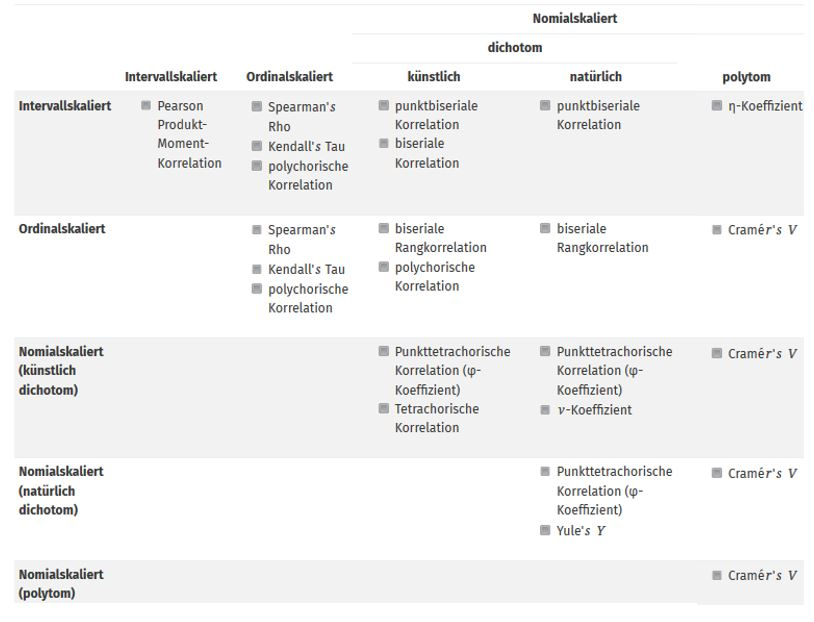
\includegraphics[width=1\textwidth,height=\textheight]{Images/Korrelationsarten.JPG}
\caption{\textbf{Abbildung 12}: verschiedene Korrelationskoeffizienten}
\end{figure}

\subsubsection*{Spearman und Kendall}\label{spearman-und-kendall}
\addcontentsline{toc}{subsubsection}{Spearman und Kendall}

Für die Berechnung des Pearson-Korrelationskoeffizienten (\(r\)) ist das Vorliegen von kontinuierlichen Variablen erforderlich. Bei \textbf{ordinalskalierten Daten} wird eine der folgenden Rangkorrelation berechnet:

\begin{enumerate}
\def\labelenumi{\arabic{enumi}.}
\tightlist
\item
  \textbf{Spearman} \(r_s\): Spearman-Rangkorrelation setzt voraus, dass Ränge gleichabständig sind\footnote{diese Voraussetzung ist eher selten erfüllt. Sie ist gleichzusetzen mit der Annahme, dass in einem Skirennen der erste, zweite, dritte, etc. Platz genaus die gleichen Zeitabstände aufweisen. Ist diese nicht gegeben, sollte Kendalls \(\tau\) verwendet werden.} und keine Ausreißer vorliegen.
\item
  \textbf{Kendall} \(\tau\): Ränge müssen nicht gleichabständig sein und Ausreißer beeinflussen diesen Korrelationskoeffizienten weit weniger als z.B. den den \(r_s\).
\end{enumerate}

Bei den Kendall-Koeffizienten unterscheidet man noch drei unterschiedliche Maße\footnote{Details zu den unterschiedlichen Kendalls-\(\tau\) sind der Literatur zu entnehmen. Weitere Betrachtungen beziehen sich auf das Kendalls-\(\tau_b\)}:

\begin{itemize}
\tightlist
\item
  Kendalls \(\tau_a\): Rangbindungen werden nicht berücksichtigt.
\item
  Kendalls \(\tau_b\): Rangbindungen werden berücksichtigt.
\item
  Kendalls \(\tau_c\): für nicht quadratische Kontingeztafeln.
\end{itemize}

Zur Veranschaulichung der verschiedenen rangbasierten Korrelationsmaße sind folgende Aufgaben zu bearbeiten:

\begin{enumerate}
\def\labelenumi{\arabic{enumi}.}
\tightlist
\item
  Berechne zuerst nochmal die Pearson-Korrelation \(r(EP,IQ)\) des bereits geladenen Datensatzes
  und rechne dann eine Spearman Korrelation. Verwende nun die Funktion \emph{cor()} des Basispakets. Vergleiche die Ergebnisse!
\item
  Vererwende die Funktion \emph{rank()} um den Variablen \emph{EP} und \emph{IQ} Ränge zuzuordnen. Speichere die Ergebnisse in \emph{EP\_Ranks} und \emph{IQ\_Ranks} und berechnen Sie anschließend eine Pearson-Korrelation. Vergleiche die Ergebnisse mit dem vorherigen Pearson-\(r\).
\end{enumerate}

\hyperref[aufgabe-spearman-lsg]{Lösung}

\subsubsection*{Biseriale Korrelation}\label{biseriale-korrelation}
\addcontentsline{toc}{subsubsection}{Biseriale Korrelation}

Biseriale Korrelationen kommen zur Anwendung, wenn ein Merkmal \textbf{Intervall}- oder \textbf{Ordinalskaliert} und das zweite Merkmal \textbf{dichotom Nominalskaliert} ist. Für das Nominalskalierte Merkmal unterscheidet man noch zwischen:

\begin{itemize}
\tightlist
\item
  \textbf{Echt dichotome Variable}: natürlich vorkommende Gruppenteilung wie z.B. wahr/falsch, männlich/weiblich, etc. Der Zusammenhang einer solchen mit einer intervallskalierten Variablen wird durch die \textbf{punktbiseriale Korrelation} beschrieben.
\item
  \textbf{Künstlich dichotome Variable}: wird eine kontinuierliche Variable in zwei Gruppen aufgeteilt, wie z.B. zwei Altersgruppen (jung, alt), oder hohe Leistungsfähigkeit vs.~niedrige Leistungsfähigkeit, etc., dann spricht man von einer künstlich dichotomen Variablen. Zusammenhänge dieser mit einer intervallskalierten Variablen werden durch die \textbf{biseriale Korrelation} beschrieben.
\end{itemize}

Kopier den folgenden Code in dein R-Script und bearbeite folgende Aufgabenstellungen:

\begin{enumerate}
\def\labelenumi{\arabic{enumi}.}
\tightlist
\item
  Verwende die Funktion \emph{dicho()} des Pakets sjmisc um alle Variablen über den Median zu dichotomisieren (\emph{Hinweise}: ersetze die \emph{XXX} im Code mit den entsprechenden Werten).
\item
  Berechne die biseriale Korrelation der Variablen \emph{IQ} und der Exam-Performance-Gruppe (\emph{EP\_Grp}).
\end{enumerate}

\begin{Shaded}
\begin{Highlighting}[]
      \CommentTok{\# Zuerst wird die Examensperformanz über den Median in zwei Gruppen geteilt}
      \CommentTok{\# library(sjmisc)}
\NormalTok{      DF\_Biserial }\OtherTok{\textless{}{-}}\NormalTok{ DF\_Korr[}\FunctionTok{order}\NormalTok{(EP), ]}
\NormalTok{      DF\_Biserial }\OtherTok{\textless{}{-}}\NormalTok{ sjmisc}\SpecialCharTok{::}\FunctionTok{dicho}\NormalTok{(XXX,}
                                   \AttributeTok{dich.by =} \StringTok{"XXX"}\NormalTok{, }
                                   \AttributeTok{as.num =} \ConstantTok{FALSE}\NormalTok{, }
                                   \AttributeTok{var.label =} \StringTok{"Grp"}\NormalTok{,}
                                   \AttributeTok{val.labels =} \FunctionTok{c}\NormalTok{(}\StringTok{"low"}\NormalTok{, }\StringTok{"high"}\NormalTok{), }
                                   \AttributeTok{append =} \ConstantTok{TRUE}\NormalTok{, }
                                   \AttributeTok{suffix =} \StringTok{"\_Grp"}\NormalTok{)}

      \FunctionTok{biserial}\NormalTok{(}\AttributeTok{x =}\NormalTok{ XXX, }\AttributeTok{y =}\NormalTok{ XXX)}
\end{Highlighting}
\end{Shaded}

\hyperref[aufgabe-biserial-lsg]{Lösung}

\subsubsection*{Phi-Koeffizient}\label{phi-koeffizient}
\addcontentsline{toc}{subsubsection}{Phi-Koeffizient}

Korrelationen zwischen echt-dichotomen Variablen (männlich/weiblich, etc.) können mit dem Phi-Koeffizienten berechnet werden. Um den Phi-Koeffizienten zu berechnen, werden Häufigkeiten in Form einer Vier-Felder-Tafel benötigt.

\begin{figure}
\centering
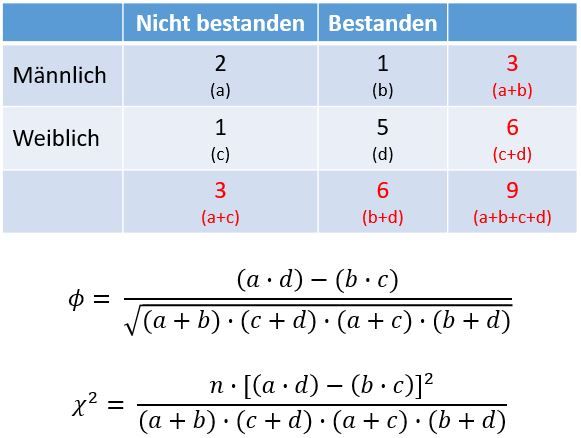
\includegraphics[width=0.7\textwidth,height=\textheight]{Images/PHIKoeffizient.JPG}
\caption{\textbf{Abbildung 13}: Beispiel und Berechnung des Phi-Koeffizienten}
\end{figure}

Folgendes einfaches Beispiel zeigt die Berechnung des Phi-Koeffizienten sowie dessen Äquivalenz mit einer Pearson-Korrelation:

\begin{Shaded}
\begin{Highlighting}[]
\NormalTok{      Geschlecht }\OtherTok{\textless{}{-}} \FunctionTok{c}\NormalTok{(}\DecValTok{1}\NormalTok{,  }\DecValTok{1}\NormalTok{,  }\DecValTok{0}\NormalTok{,  }\DecValTok{0}\NormalTok{,  }\DecValTok{1}\NormalTok{,  }\DecValTok{0}\NormalTok{,  }\DecValTok{1}\NormalTok{,  }\DecValTok{1}\NormalTok{,  }\DecValTok{1}\NormalTok{)}
\NormalTok{      Bestanden  }\OtherTok{\textless{}{-}} \FunctionTok{c}\NormalTok{(}\DecValTok{1}\NormalTok{,  }\DecValTok{1}\NormalTok{,  }\DecValTok{1}\NormalTok{,  }\DecValTok{0}\NormalTok{,  }\DecValTok{0}\NormalTok{,  }\DecValTok{0}\NormalTok{,  }\DecValTok{1}\NormalTok{,  }\DecValTok{1}\NormalTok{,  }\DecValTok{1}\NormalTok{)}
      
\NormalTok{      VFT        }\OtherTok{\textless{}{-}} \FunctionTok{table}\NormalTok{(Geschlecht, Bestanden)}
\NormalTok{      pander}\SpecialCharTok{::}\FunctionTok{pander}\NormalTok{(VFT)}
      
      \FunctionTok{cor}\NormalTok{(Geschlecht, Bestanden)}
      
      \FunctionTok{phi}\NormalTok{(VFT)}
\NormalTok{      CST }\OtherTok{\textless{}{-}} \FunctionTok{chisq.test}\NormalTok{(VFT, }\AttributeTok{correct =} \ConstantTok{FALSE}\NormalTok{)}
\NormalTok{      pander}\SpecialCharTok{::}\FunctionTok{pander}\NormalTok{(CST)}
      \FunctionTok{qchisq}\NormalTok{(}\AttributeTok{p=}\NormalTok{.}\DecValTok{95}\NormalTok{,}\AttributeTok{df=}\DecValTok{1}\NormalTok{) }\CommentTok{\# kritischer Chi{-}Square{-}Wert bei einem Freiheitsgrad und Alpha = 5\%}
\end{Highlighting}
\end{Shaded}

Die Anzahl der Freiheitsgrade beträgt in diesem Fall immer eins, da wir es mit zwei dichotomen Merkmalen zu tun haben.

\subsubsection*{Tetrachorische Korrelation}\label{tetrachorische-korrelation}
\addcontentsline{toc}{subsubsection}{Tetrachorische Korrelation}

Soll der Zusammenhang zwischen zwei künstlich-dichotomen Variablen berechnet werden, die aus stetigen, normalverteilten latente Variablen abgeleitet wurden (z.B. Intelligenz und Examperformanz in Statistik), verwendet man die tetrachorische Korrelation.

Auf Details zur Berechnung der Kenngröße wird hier verzichtet. Grundlage ist wiederum eine Vier-Felder-Tafel (wie beim Phi-Koeffizienten), wobei die tetrachorische Korrelation nicht so stark von der Randverteilung der Vier-Felder-Tafel abhängt. Zu beachten ist jedoch, dass die Zellbesetzung von b und c nicht 0 sein darf! Nachfolgendes Beispiel sollte die Anwendung der tetrachorischen Korrelation verdeutlichen. Lade dazu den folgenden Code und führe diesen Zeilenweise aus. Diskutiere die Ergebnisse!

\begin{Shaded}
\begin{Highlighting}[]
      \CommentTok{\# library (psych) }
      \FunctionTok{load}\NormalTok{(}\StringTok{"Daten/TetraCorrBsp.Rda"}\NormalTok{)}
\NormalTok{      TCC\_Res }\OtherTok{\textless{}{-}} \FunctionTok{tetrachoric}\NormalTok{(DF\_TCC)}
      \FunctionTok{pander}\NormalTok{(TCC\_Res}\SpecialCharTok{$}\NormalTok{rho)}
\end{Highlighting}
\end{Shaded}

\subsubsection*{Polychorische Korrelation}\label{polychorische-korrelation}
\addcontentsline{toc}{subsubsection}{Polychorische Korrelation}

Um Korrelationen zwischen ordinalen Daten zu beschreiben, verwendet man die polychorische Korrelation. Dabei schätzt man die Korrelation zwischen zwei (ordinalen) Merkmalen, die in mehr als zwei geordnete Kategorien unterteilt sind. Die Berechnung ist überaus komplex und wird hier nicht dargestellt.

Polychorische Korrelationen werden unter anderem verwendet, um konfirmatorische Faktorenanalysen mit ordinalen Daten zu berechnen. Es ist mit Programmen wie R, AMOS, LISREL oder MPlus auch möglich, exploratorische Faktorenanalysen mit polychorischen Korrelationen durchzuführen.

Betrachte folgendes Beispiel:

\begin{Shaded}
\begin{Highlighting}[]
    \FunctionTok{library}\NormalTok{(polycor)}
    \FunctionTok{library}\NormalTok{(mvtnorm)}
    \FunctionTok{set.seed}\NormalTok{(}\DecValTok{12345}\NormalTok{)}
\NormalTok{    data }\OtherTok{\textless{}{-}} \FunctionTok{rmvnorm}\NormalTok{(}\DecValTok{1000}\NormalTok{, }\FunctionTok{c}\NormalTok{(}\DecValTok{0}\NormalTok{, }\DecValTok{0}\NormalTok{), }\FunctionTok{matrix}\NormalTok{(}\FunctionTok{c}\NormalTok{(}\DecValTok{1}\NormalTok{, .}\DecValTok{5}\NormalTok{, .}\DecValTok{5}\NormalTok{, }\DecValTok{1}\NormalTok{), }\DecValTok{2}\NormalTok{, }\DecValTok{2}\NormalTok{))}
    \CommentTok{\# Pearson correlation of those data points.}
    \FunctionTok{cor}\NormalTok{(data) }\CommentTok{\# 0.5264}
    \CommentTok{\# And the Spearman correlation  }
    \FunctionTok{cor}\NormalTok{(data, }\AttributeTok{method=}\StringTok{"spearman"}\NormalTok{) }\CommentTok{\#0.5043}
    \CommentTok{\# Now let’s try with polychoric correlation.}
    \CommentTok{\# First we need some cutoffs to break the data into cells ideally with breakpoints that avoid nearly empty cells.}
\NormalTok{    x }\OtherTok{\textless{}{-}} \FunctionTok{cut}\NormalTok{(data[,}\DecValTok{1}\NormalTok{], }\FunctionTok{c}\NormalTok{(}\SpecialCharTok{{-}}\ConstantTok{Inf}\NormalTok{, .}\DecValTok{75}\NormalTok{, }\ConstantTok{Inf}\NormalTok{))}
\NormalTok{    y }\OtherTok{\textless{}{-}} \FunctionTok{cut}\NormalTok{(data[,}\DecValTok{2}\NormalTok{], }\FunctionTok{c}\NormalTok{(}\SpecialCharTok{{-}}\ConstantTok{Inf}\NormalTok{, }\SpecialCharTok{{-}}\DecValTok{1}\NormalTok{, .}\DecValTok{5}\NormalTok{, }\FloatTok{1.5}\NormalTok{, }\ConstantTok{Inf}\NormalTok{))}
    \CommentTok{\# Then take the polychoric correlation.}
    \CommentTok{\# The default method uses the faster 2{-}step method and only returns the correlation.}
    \FunctionTok{polychor}\NormalTok{(x, y)}
    \CommentTok{\# You don’t need all the multivariate random normal overhead, polychor() works on any crosstab.}
\NormalTok{    tab }\OtherTok{\textless{}{-}} \FunctionTok{table}\NormalTok{(x,y)    }
    \FunctionTok{polychor}\NormalTok{(tab)}
    \CommentTok{\# Let’s try the same data with some different cutoffs and see how it does}
\NormalTok{    x2 }\OtherTok{\textless{}{-}} \FunctionTok{cut}\NormalTok{(data[,}\DecValTok{1}\NormalTok{], }\FunctionTok{c}\NormalTok{(}\SpecialCharTok{{-}}\ConstantTok{Inf}\NormalTok{, }\SpecialCharTok{{-}}\DecValTok{2}\NormalTok{, }\SpecialCharTok{{-}}\DecValTok{1}\NormalTok{, }\DecValTok{0}\NormalTok{, }\DecValTok{1}\NormalTok{, }\DecValTok{2}\NormalTok{, }\ConstantTok{Inf}\NormalTok{))}
\NormalTok{    y2 }\OtherTok{\textless{}{-}} \FunctionTok{cut}\NormalTok{(data[,}\DecValTok{2}\NormalTok{], }\FunctionTok{c}\NormalTok{(}\SpecialCharTok{{-}}\ConstantTok{Inf}\NormalTok{, }\SpecialCharTok{{-}}\DecValTok{2}\NormalTok{, }\SpecialCharTok{{-}}\DecValTok{1}\NormalTok{, }\DecValTok{0}\NormalTok{, }\DecValTok{1}\NormalTok{, }\DecValTok{2}\NormalTok{, }\ConstantTok{Inf}\NormalTok{))}
    \FunctionTok{table}\NormalTok{(x2,y2)    }
    \FunctionTok{polychor}\NormalTok{(x2,y2,}\AttributeTok{ML=}\ConstantTok{TRUE}\NormalTok{,}\AttributeTok{std.err=}\ConstantTok{TRUE}\NormalTok{)}
\end{Highlighting}
\end{Shaded}

\section*{Lösungen}\label{luxf6sungen}
\addcontentsline{toc}{section}{Lösungen}

\subsection*{Aufgabe Korrelation Lsg}\label{aufgabe-korrelation-lsg}
\addcontentsline{toc}{subsection}{Aufgabe Korrelation Lsg}

\begin{Shaded}
\begin{Highlighting}[]
  \CommentTok{\# library(Hmisc) für Hmisc::rcorr}
  \CommentTok{\# library(corrplot) für corrplot}
  \CommentTok{\# library(pwr)}
  
  \CommentTok{\# 1. Ermitteln Sie mit einer geeigneten Funktion die Korrelationen und prüfen Sie }
  \CommentTok{\#    diese auch auf statistische Signifikanz.}
\NormalTok{    CorRes }\OtherTok{\textless{}{-}}\NormalTok{ Hmisc}\SpecialCharTok{::}\FunctionTok{rcorr}\NormalTok{(}\FunctionTok{as.matrix}\NormalTok{(DF\_Korr), }\AttributeTok{type=}\StringTok{"pearson"}\NormalTok{) }\CommentTok{\# type can be pearson or spearman}
\NormalTok{    pander}\SpecialCharTok{::}\FunctionTok{pander}\NormalTok{(}\FunctionTok{round}\NormalTok{(CorRes}\SpecialCharTok{$}\NormalTok{r, }\DecValTok{2}\NormalTok{))}
\NormalTok{    pander}\SpecialCharTok{::}\FunctionTok{pander}\NormalTok{(}\FunctionTok{round}\NormalTok{(CorRes}\SpecialCharTok{$}\NormalTok{P , }\DecValTok{2}\NormalTok{))}
  \CommentTok{\# 2. Zeichnen Sie einen Korrelationsplot mit dem Paket *corrplot*.}
\NormalTok{    corrplot}\SpecialCharTok{::}\FunctionTok{corrplot}\NormalTok{(}\FunctionTok{cor}\NormalTok{(DF\_Korr), }\AttributeTok{type=}\StringTok{"upper"}\NormalTok{, }\AttributeTok{method =} \StringTok{"ellipse"}\NormalTok{)}
  \CommentTok{\# 3. Berechnen Sie die Teststärke der Korrelation $r(IQ, EP)$}
  \CommentTok{\#    (Hinweis: verwenden Sie die Funktion *pwr::pwr.r.test* des Pakets *pwr*).}
\NormalTok{    N    }\OtherTok{\textless{}{-}} \FunctionTok{dim}\NormalTok{(DF\_Korr)[}\DecValTok{1}\NormalTok{]}
\NormalTok{    PwrA }\OtherTok{\textless{}{-}}\NormalTok{ pwr}\SpecialCharTok{::}\FunctionTok{pwr.r.test}\NormalTok{(}\AttributeTok{n =}\NormalTok{ N, }\AttributeTok{r =} \FloatTok{0.47}\NormalTok{, }\AttributeTok{sig.level =} \FloatTok{0.05}\NormalTok{, }\AttributeTok{alternative =} \StringTok{\textquotesingle{}two.sided\textquotesingle{}}\NormalTok{)}
\NormalTok{    pander}\SpecialCharTok{::}\FunctionTok{pander}\NormalTok{(}\FunctionTok{data.frame}\NormalTok{(}\AttributeTok{Kennwerte =} \FunctionTok{unlist}\NormalTok{(PwrA)))}
  \CommentTok{\# 4. Verwenden diese Funktion (*pwr::pwr.r.test*) um für eine Korrelation $r(x,y) = 0.21$ }
  \CommentTok{\#    den optimalen Stichprobenumfang zu berechnen.  }
\NormalTok{    OptN }\OtherTok{\textless{}{-}}\NormalTok{ pwr}\SpecialCharTok{::}\FunctionTok{pwr.r.test}\NormalTok{(}\AttributeTok{r =} \FloatTok{0.21}\NormalTok{, }\AttributeTok{sig.level =} \FloatTok{0.05}\NormalTok{, }\AttributeTok{power =} \FloatTok{0.95}\NormalTok{, }\AttributeTok{alternative =} \StringTok{\textquotesingle{}greater\textquotesingle{}}\NormalTok{)}
\NormalTok{    pander}\SpecialCharTok{::}\FunctionTok{pander}\NormalTok{(}\FunctionTok{data.frame}\NormalTok{(}\AttributeTok{Kennwerte =} \FunctionTok{unlist}\NormalTok{(OptN)))}
  \CommentTok{\# 5. Prüfen Sie mit Hilfe der Funktion *mvn* aus dem Paket *MVN* }
  \CommentTok{\#    die Voraussetzung der bivariaten Normalverteilung der }
  \CommentTok{\#    Variablenpaare (EP,IQ), (EP, VZ) und (EP,PA).}
    \CommentTok{\# library(MVN)}
    \CommentTok{\# mvn(DF\_Korr[, c("EP","IQ")], multivariatePlot = "persp")}
    \CommentTok{\# mvn(DF\_Korr[, c("EP","VZ")], multivariatePlot = "persp")}
    \CommentTok{\# mvn(DF\_Korr[, c("EP","PA")], multivariatePlot = "persp")}

  \CommentTok{\# 6. Berechnen Sie die durchschnittliche Korrelation von $r\_1(EP,IQ)$, $r\_1(EP,VZ)$ und $r\_1(EP,PA)$.}
      \FunctionTok{round}\NormalTok{(}\FunctionTok{fisherz2r}\NormalTok{(}\FunctionTok{mean}\NormalTok{(}\FunctionTok{c}\NormalTok{(}\FunctionTok{fisherz}\NormalTok{(.}\DecValTok{47}\NormalTok{), }\FunctionTok{fisherz}\NormalTok{(.}\DecValTok{36}\NormalTok{), }\FunctionTok{fisherz}\NormalTok{(}\SpecialCharTok{{-}}\NormalTok{.}\DecValTok{25}\NormalTok{)))), }\DecValTok{2}\NormalTok{)}
  \CommentTok{\# 7. Prüfen Sie, on der Unterschied der Korrelationskoeffizienten $r(EP,IQ) = 0.47$ und $r(EP,VZ) = 0.36$}
  \CommentTok{\#    statistisch signifikant ist. Verwenden Sie die Funktion *psych::paired.r()* aus dem Paket *psych*}
    \CommentTok{\# library(psych)}
\NormalTok{    psych}\SpecialCharTok{::}\FunctionTok{paired.r}\NormalTok{(}\AttributeTok{xy        =}\NormalTok{ .}\DecValTok{47}\NormalTok{, }
             \AttributeTok{xz        =}\NormalTok{ .}\DecValTok{36}\NormalTok{, }
             \AttributeTok{n         =}\NormalTok{ N,}
             \AttributeTok{twotailed =} \ConstantTok{TRUE}\NormalTok{) }
\end{Highlighting}
\end{Shaded}

\hyperref[aufgabe-korrelation]{zurück zu Aufgabe}

\subsection*{Aufgabe Spearman Lsg}\label{aufgabe-spearman-lsg}
\addcontentsline{toc}{subsection}{Aufgabe Spearman Lsg}

\begin{Shaded}
\begin{Highlighting}[]
    \CommentTok{\# library(Hmisc)}

    \CommentTok{\# 1. Berechnen Sie zuerst nochmal die Pearson{-}Korrelation $r(EQ,IQ)$ des bereits geladenen Datensatzes}
    \CommentTok{\#    und rechnen Sie dann eine Spearman Korrelation. Verwenden Sie nun die Funktion cor() des Basispakets.}
    \CommentTok{\#    Vergleichen Sie die Ergebnisse!}
    
\NormalTok{    EP }\OtherTok{\textless{}{-}}\NormalTok{ DF\_Korr}\SpecialCharTok{$}\NormalTok{EP}
\NormalTok{    IQ }\OtherTok{\textless{}{-}}\NormalTok{ DF\_Korr}\SpecialCharTok{$}\NormalTok{IQ}
    
\NormalTok{    CorPearson  }\OtherTok{\textless{}{-}} \FunctionTok{round}\NormalTok{(}\FunctionTok{cor}\NormalTok{(EP, IQ, }\AttributeTok{method =} \StringTok{"pearson"}\NormalTok{), }\DecValTok{2}\NormalTok{)}
\NormalTok{    CorSpearman }\OtherTok{\textless{}{-}} \FunctionTok{round}\NormalTok{(}\FunctionTok{cor}\NormalTok{(EP, IQ, }\AttributeTok{method =} \StringTok{"spearman"}\NormalTok{), }\DecValTok{2}\NormalTok{)}
\NormalTok{    CorKendall  }\OtherTok{\textless{}{-}} \FunctionTok{round}\NormalTok{(}\FunctionTok{cor}\NormalTok{(EP, IQ, }\AttributeTok{method =} \StringTok{"kendall"}\NormalTok{), }\DecValTok{2}\NormalTok{)}
    
\NormalTok{    pander}\SpecialCharTok{::}\FunctionTok{pander}\NormalTok{(}\FunctionTok{data.frame}\NormalTok{(}\AttributeTok{Pearson  =}\NormalTok{ CorPearson,}
                      \AttributeTok{Spearman =}\NormalTok{ CorSpearman,}
                      \AttributeTok{Kendall  =}\NormalTok{ CorKendall))}
    \CommentTok{\# Alternativ kann auch cor.test() verwendet werden, dabei werden die Tests auf}
    \CommentTok{\# Signigikanz gleich mitgerechnet.}
    \CommentTok{\# cor.test(x = EP, }
    \CommentTok{\#          y = IQ, }
    \CommentTok{\#          alternative = \textquotesingle{}two.sided\textquotesingle{}, }
    \CommentTok{\#          method = \textquotesingle{}pearson\textquotesingle{})    }
    \CommentTok{\# cor.test(x = EP, }
    \CommentTok{\#          y = IQ, }
    \CommentTok{\#          alternative = \textquotesingle{}two.sided\textquotesingle{}, }
    \CommentTok{\#          method = \textquotesingle{}spearman\textquotesingle{})    }
    \CommentTok{\# cor.test(x = EP, }
    \CommentTok{\#          y = IQ, }
    \CommentTok{\#          alternative = \textquotesingle{}two.sided\textquotesingle{}, }
    \CommentTok{\#          method = \textquotesingle{}kendall\textquotesingle{})    }
    \CommentTok{\# Bemerkung: cor.test() mit Kendall bringt Warnung bezüglich der Rangbindungen.}
    \CommentTok{\#            Alternativ kann man daher die Funktion Kendall() des Paketes Kendal verwenden:}
      \CommentTok{\# library(Kendall)}
        \CommentTok{\# Kendall(x = EP, }
        \CommentTok{\#         y = IQ)}
    \CommentTok{\# 2. Verwenden Sie die Funktion rank() um den Variablen EP und IQ Ränge zuzuordnen.}
    \CommentTok{\#   Speichern Sie die Ergebnisse in EP\_Ranks und IQ\_Ranks und berechnen Sie anschließend}
    \CommentTok{\#   eine Pearson{-}Korrelation. Vergleichen Sie die Ergebnisse mit dem vorherigen Pearson{-}r.}
\NormalTok{    EP\_Ranks }\OtherTok{\textless{}{-}} \FunctionTok{rank}\NormalTok{(EP, }\AttributeTok{na.last =} \ConstantTok{TRUE}\NormalTok{,}
                     \AttributeTok{ties.method =} \FunctionTok{c}\NormalTok{(}\StringTok{"average"}\NormalTok{))}
\NormalTok{    IQ\_Ranks }\OtherTok{\textless{}{-}} \FunctionTok{rank}\NormalTok{(IQ, }\AttributeTok{na.last =} \ConstantTok{TRUE}\NormalTok{,}
                     \AttributeTok{ties.method =} \FunctionTok{c}\NormalTok{(}\StringTok{"average"}\NormalTok{))}
    \FunctionTok{round}\NormalTok{(}\FunctionTok{cor}\NormalTok{(EP\_Ranks, IQ\_Ranks, }\AttributeTok{method =} \StringTok{"pearson"}\NormalTok{), }\DecValTok{2}\NormalTok{)}
\end{Highlighting}
\end{Shaded}

\hyperref[spearman-und-kendall]{zurück zu Aufgabe}

\subsection*{Aufgabe Biserial Lsg}\label{aufgabe-biserial-lsg}
\addcontentsline{toc}{subsection}{Aufgabe Biserial Lsg}

\begin{Shaded}
\begin{Highlighting}[]
    \CommentTok{\# Zuerst wird die Examensperformanz über den Median in zwei Gruppen geteilt}
    \CommentTok{\# library(sjmisc)}
\NormalTok{    DF\_Biserial }\OtherTok{\textless{}{-}}\NormalTok{ DF\_Korr[}\FunctionTok{order}\NormalTok{(EP), ]}
\NormalTok{    DF\_Biserial }\OtherTok{\textless{}{-}}\NormalTok{ sjmisc}\SpecialCharTok{::}\FunctionTok{dicho}\NormalTok{(DF\_Biserial,}
                         \AttributeTok{dich.by =} \StringTok{"median"}\NormalTok{, }
                         \AttributeTok{as.num =} \ConstantTok{FALSE}\NormalTok{, }
                         \AttributeTok{var.label =} \StringTok{"Grp"}\NormalTok{,}
                         \AttributeTok{val.labels =} \FunctionTok{c}\NormalTok{(}\StringTok{"low"}\NormalTok{, }\StringTok{"high"}\NormalTok{), }
                         \AttributeTok{append =} \ConstantTok{TRUE}\NormalTok{, }
                         \AttributeTok{suffix =} \StringTok{"\_Grp"}\NormalTok{)}
\NormalTok{    IQ          }\OtherTok{\textless{}{-}}\NormalTok{ DF\_Biserial}\SpecialCharTok{$}\NormalTok{IQ}
    
    \FunctionTok{biserial}\NormalTok{(}\AttributeTok{x =}\NormalTok{ IQ, }\AttributeTok{y =}\NormalTok{ DF\_Biserial}\SpecialCharTok{$}\NormalTok{EP\_Grp)    }

\CommentTok{\# https://www.r{-}bloggers.com/2021/02/how{-}does{-}polychoric{-}correlation{-}work{-}aka{-}ordinal{-}to{-}ordinal{-}correlation/}
\end{Highlighting}
\end{Shaded}

\hyperref[biseriale-korrelation]{zurück zu Aufgabe}

\end{document}
